\chapter{Codifica di canale}
Tratteremo ora il caso di una trasmissione, in cui sia presente il rumore. In altre parole non è certo che quello che viene inviato, 
corrisponda a quello che viene ricevuto. Si tratta in sostanza dello schema in figura \ref{fig:0007}.
In questo caso quindi (diversamente dalla codifica di sorgente) non siamo interessati a comprimere l'informazione. Vogliamo invece 
aggiungere della ridondanza, al fine di aumentare l'affidabilità della trasmissione.
Cercheremo infine di trovare un compromesso tra affidabilità ed efficienza.

\section{Capacità di canale}
Fino ad ora non abbiamo definito in maniera formale un canale di trasmissione. Tuttavia, come vedremo, si tratta di un concetto fondamentale. Per fare un esempio, l'affidabilità e l'efficienza che si possono raggiungere dipendono strettamente dal canale.
E' quindi utile definirlo con precisione, unitamente a concetti come la sua capacità.

\begin{definizione}[Canale]
 Un canale $\mathcal{C}$ è una terna $\mathcal{C}=(X,p(y/x),Y)$. Dove:
 \begin{itemize}
  \item $X$ è l'alfabeto di ingresso
  \item $p(y/x)$ sono le probabilità forward. Ovvero $p(y_i/x_j)$ è la probabilità che il destinatario 
        abbia ricevuto $y_i$, quanto è stato inviato $x_j$.
  \item $Y$ è l'alfabeto di uscita
 \end{itemize}
\end{definizione}

\noindent
Per rappresentare un canale (e quindi le tre quantità appena indicate), si utilizzano fondamentalmente due modalità:
\begin{itemize}
 \item \textbf{Matrice di canale}: E' una matrice $|X| \times |Y|$, che contiene le probabilità forward.
                          Ovvero in posizione $(i,j)$ è riportata $p(y_j/x_i)$. (Esempio in figura \ref{fig:noiseless2}).
 \item \textbf{Grafo di canale}: E' un grafo bipartito: un insieme di nodi è formato da $X_1,X_2,..,X_n$, l'altro insieme 
                        da $Y_1,Y_2,...,Y_m$.
                        Gli archi che connettono i nodi sono etichettati con le probabilità forward. Ovvero l'arco che connette
                        $X_i$ con $Y_j$ riporta $p(y_j/x_i)$. Per convenzione, se per qualche i,j $p(y_j/x_i)=0$, l'arco viene omesso.
                       (Esempio in figura \ref{fig:noiseless1}).
\end{itemize}

\bigskip

\begin{definizione}[Estensione di un canale]
 Dato un canale $\mathcal{C}(X,p(y/x),Y)$ la sua estensione n-esima è:
\[
 C^n=(X^n,p^n(y,x),Y^n)
\]
Dove:
\begin{itemize}
 \item $X^n=X \times X \times ... \times X$
 \item $Y^n=Y \times Y \times ... \times Y$
 \item $p^n(y,x)=\prod_{i=1}^n p(y_i/x_i)$ (se il canale è senza memoria)
\end{itemize}
\end{definizione}

\bigskip

Da qui in avanti assumeremo sempre di trovarci in presenza di un canale ``senza memoria''. Ovvero in un canale dove la probabilità 
di emissione di un simbolo, non dipende dai simboli emessi precedentemente ma unicamente dal simbolo inviato.
Fatte queste premesse, siamo ora interessati a calcolare la capacità informazionale di un canale. Vogliamo in sostanza determinare 
la massima quantità di informazione che può viaggiare attraverso un canale. Se ci mettiamo dalla parte del destinatario, inizialmente 
non abbiamo visto arrivare alcun simbolo dal canale. Pertanto la nostra ``incertezza'' sulla variabile $X$ è l'entropia $H(X)$. Dopo l'arrivo di un simbolo però, la nostra incertezza si riduce ad $H(X/Y)$. E' in sostanza l'incertezza che ci rimane su X, dopo aver 
visto Y. L'informazione che ha viaggiato sul canale è dunque:
\[
 H(X)-H(X/Y)=I(X;Y)
\]

La massima quantità di informazione che può viaggiare attraverso un canale, sarà dunque data dal massimo valore che può 
assumere l'informazione mutua. Vediamo allora da cosa dipende questo valore:
\[\begin{split}
 I(X;Y)=&H(X)-H(X/Y) \\
        =&\sum_{x \in X} \sum_{y \in Y} p(x,y) log \frac{p(x,y)}{p(x)p(y)} \\
        =&\sum_{x \in X} \sum_{y \in Y} p(x)p(y/x) log \frac{p(x)p(y/x)}{p(x)p(y)} \\
        =&\sum_{x \in X} \sum_{y \in Y} p(x)p(y/x) log \frac{p(y/x)}{p(y)} \\
        =&\sum_{x \in X} \sum_{y \in Y} p(x)p(y/x) log \frac{p(y/x)}{ \displaystyle\sum_{z \in X} p(z)p(y/z)} \\
  \end{split}
\]

Come si nota dall'ultimo risultato, l'informazione mutua dipende dalle probabilità forward (termini $p(y/x)$ e $p(y/z)$) e dalle probabilità di ``ingresso'' (termini $p(x)$ e $p(z)$).
Possiamo in sostanza dire che:
\[
 I(X;Y)=f(S,C)
\]
Ovvero l'informazione mutua è una funzione della sorgente e del canale. Visto che vogliamo calcolare la capacità di uno specifico canale, non potremo variare le probabilità forward. In altre parole, le probabilità forward sono una caratteristica specifica del canale, sulle quali non si può agire. Pertanto per calcolare il massimo dell'informazione mutua (come detto poco prima), potremo agire 
unicamente sulle probabilità di ``ingresso''. Questo ci porta direttamente alla definizione di capacità di canale.

\begin{definizione}
 La capacità di un canale (senza memoria) è:
 \[
  C=\max_{p(x)} I(X;Y)
 \]

\end{definizione}

\bigskip

\noindent
Vediamo ora alcune proprietà della capacità di canale.

\begin{osservazione}
\[
 C \ge 0
\]
 \begin{proof}
  \[
   C=\max_{p(x)} I(X;Y)
  \]
  Ma $I(X;Y) \ge 0$ (Osservazione \ref{distinf}).
 \end{proof}
\end{osservazione}

\bigskip

\begin{osservazione}
\[
 C \le min\{log(|X|), log(|Y|)\}
\]
 \begin{proof}
  \[
   I(X;Y)=H(X)-H(X/Y) \le H(X) \le log(|X|)
  \]
  E:
  \[
   I(X;Y)=H(Y)-H(Y/X) \le H(Y) \le log(|Y|)
  \]
  Da cui $I(X;Y) \le min\{log(|X|), log(|Y|)\}$
 \end{proof}
\end{osservazione}

\bigskip

\begin{osservazione}
\mbox{}

 I(X;Y) è continua in p(x)
\end{osservazione}

\begin{osservazione}
\mbox{}

 I(X;Y) è concava in p(x)
\begin{proof}
\mbox{}

 \noindent
 Osserviamo che se $f$ è una funzione concava e $g$ è una funzione lineare. Ovvero (in simboli):
 \[
  f(\lambda x+(1-\lambda)y) \ge \lambda f(x)+ (1-\lambda) f(y) \ \ \forall \lambda \in [0,1]
 \]
 \[
  g(ax+by)=ag(x)+bg(y)
 \] 
  Allora:
  \begin{itemize}
   \item[a)] $h=f \circ g$ è concava. Infatti:
              \[\begin{split}
              h(\lambda x + (1-\lambda)y)&=f(g(\lambda x + (1-\lambda)y)) \\
              &=f(\lambda g(x) + (1-\lambda)g(y)) \\
              & \ge \lambda f(g(x)) + (1-\lambda)f(g(y)) \\
              &=\lambda h(x) + (1-\lambda)h(y) \\
               \end{split}
             \]

   \item[b)] $h=f+g$ è concava. Infatti:
              \[\begin{split}
                h(\lambda x + (1-\lambda)y)&=f(\lambda x + (1-\lambda)y)+g(\lambda x + (1-\lambda)y) \\
                &\ge \lambda f(x) + (1-\lambda)f(y)+g(\lambda x + (1-\lambda)y) \\
                &=\lambda f(x) + (1-\lambda)f(y)+ \lambda g(x) + (1-\lambda)g(y) \\
                &=\lambda[f(x)+g(x)] + (1-\lambda)[f(y)+g(y)] \\
                &=\lambda h(x) + (1-\lambda)h(y) \\
               \end{split}
              \]

  \end{itemize}
  Ora, per il teorema \ref{infmutua}:
  \[
   I(X;Y)=H(Y)-H(Y/X)
  \]
  $H(Y)$ è concava rispetto a $p(y)$. Inoltre:
  \[
   p(y)=\sum_{x \in X}p(x)p(y/x)
  \]
   Quindi $p(y)$ è lineare rispetto a $p(x)$. Quindi per (a), $H(Y)$ è concava rispetto a $p(x)$.
  Esaminiamo ora $H(Y/X)$.
  \[
   H(Y/X)=\sum_{x \in X} p(x)H(Y/X=x)
  \]
   Ma $H(Y/X=x)$ non dipende da $p(x)$, quindi $H(Y/X)$ è lineare in $p(x)$.
   Ora per (b), la somma di una funzione concava e di una lineare da una funzione concava, concludendo la dimostrazione.
\end{proof}
\end{osservazione}
Nota: le ultime due proprietà non riguardano la capacità di canale, ma l'informazione mutua. Tuttavia sono strettamente legate alla 
capacità di canale (visto che è appunto il massimo dell'informazione mutua).

\section{Tipi di canali}
Vediamo ora alcune famiglie di canali, unitamente alla loro capacità.
Successivamente presentiamo anche 3 particolari canali (sempre studiando la loro capacità).

\subsection{Canale noiseless}

\medskip

\begin{definizione}
 Un canale si dice noiseless (uno a molti) se:
\[
 \forall y \in Y \exists ! \ x \in X \ : \ p(y/x) > 0
\]
\end{definizione}

In questo tipo di canale quindi, il destinatario sa sempre che simbolo è stato inviato.
Il mittente invece non è in grado di sapere cosa il destinatario abbia ricevuto.
In figura \ref{fig:noiseless} è riportato un esempio di canale noiseless.

\begin{figure}[htbp]
  \centering
  \subfloat[Grafo di canale]{\label{fig:noiseless1}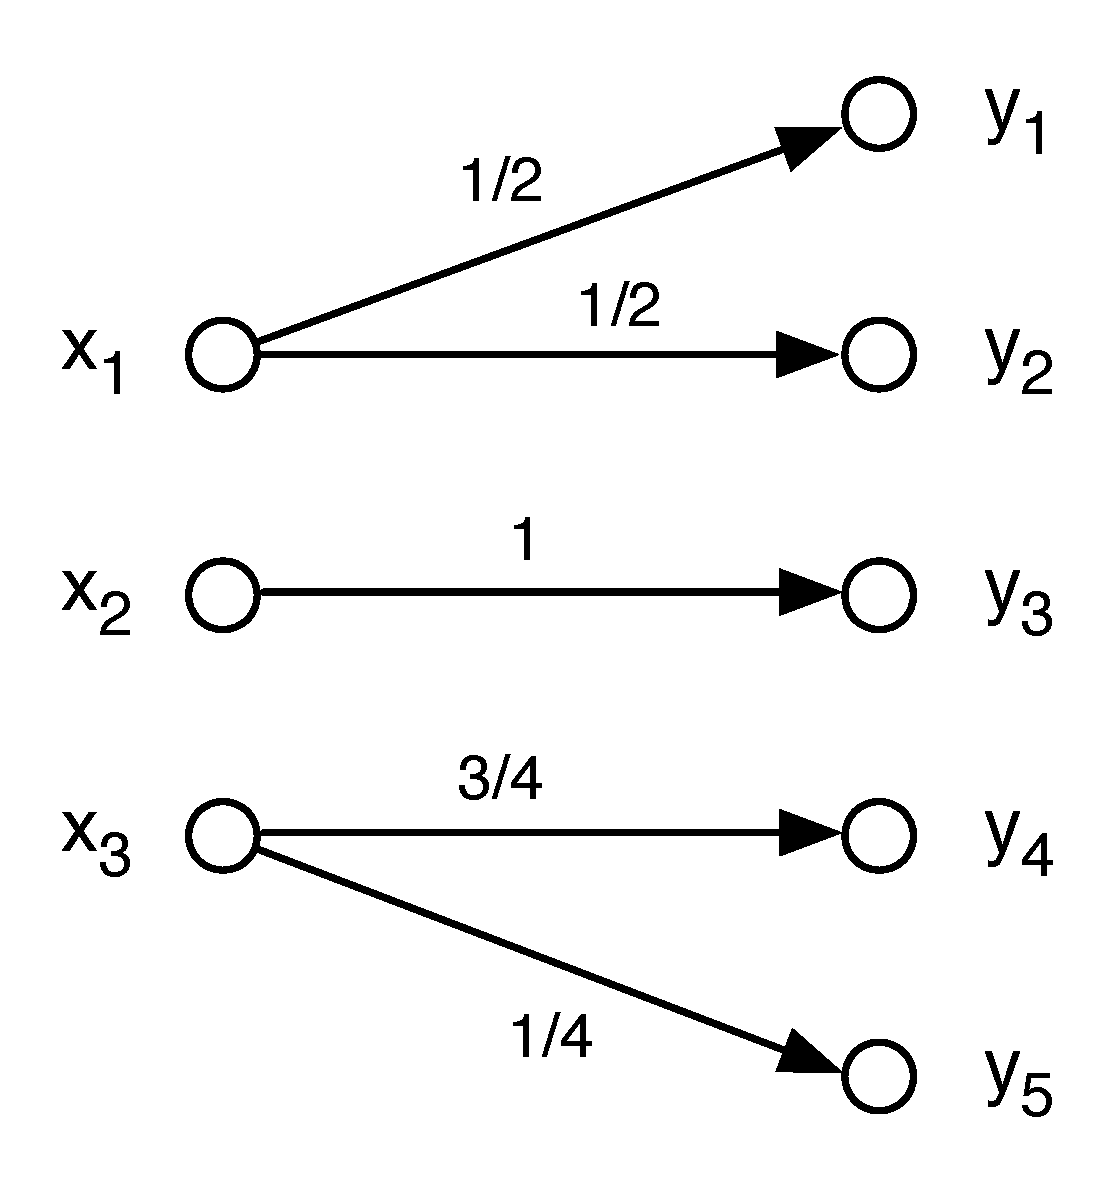
\includegraphics[width=0.4\textwidth]{img/noiseless1.pdf}}        
  \hspace{1cm}
  \subfloat[Matrice di canale]{\label{fig:noiseless2}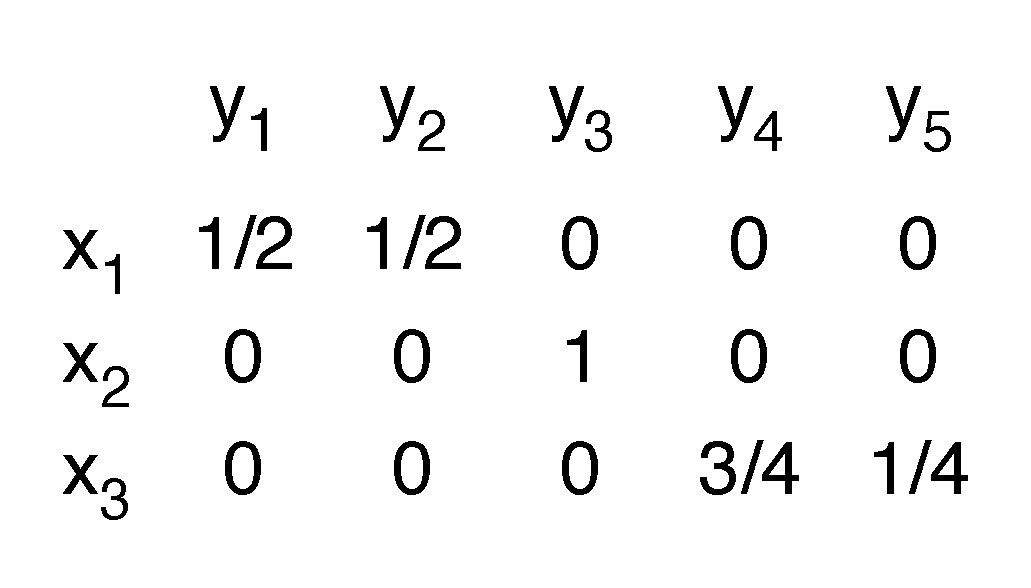
\includegraphics[width=0.4\textwidth]{img/noiseless2.pdf}}
  \caption{Esempio di canale noiseless}
  \label{fig:noiseless}
\end{figure}

\begin{lemma}
 Se $\C$ è noisless, allora $H(X/Y)=0$
 \begin{proof}
 Supponiamo per comodità
 che $\forall y \in Y p(y)>0$. Se così non fosse, sarebbe sufficiente rimuovere il simbolo (non c'è quindi perdita di generalità).
 Dalla definizione di entropia condizionata:
 \[
  H(X/Y)=\sum_{y \in Y} p(y)H(X/Y=y)
 \]
 Poiché abbiamo supposto $p(y)>0$, bisogna dimostrare che:
 \[
  \forall y \in Y \ : \ H(X/Y=y)=\sum_{x \in X}p(x/y) log( p(x/y)) =0
 \]
 Chiaramente l'uguaglianza vale se: 
 \[
  \forall x \in X, \forall y \in Y \ : \ p(x/y)=0 \lor p(x/y)=1
 \]
 In maniera intuitiva però ciò è vero, è sufficiente infatti osservare il grafo di canale. Preso un certo $y$, esiste un unico 
 arco che lo connette ad un certo $x$ (il caso con probabilità 1), mentre nessun arco che lo connette ad altri $x$ (i casi con 
 probabilità 0).
 In maniera più formale, chiamiamo $x(y)$ l'unico $x$ per cui $p(y/x)>0$ (ne esiste uno solo per la def. di canale noiseless).
 Ora:
 \[
  p(x/y)=\frac{p(y/x)p(x)}{p(y)}=\frac{p(y/x)p(x)}{ \displaystyle\sum_{z \in X} p(y/z)p(z)}=
  \frac{p(y/x)p(x)}{ p(y/x(y))p(x(y))}
 \]
 A questo punto se x=x(y) si ottiene:
 \[
  p(x(y)/y)=\frac{p(y/x(y))p(x(y))}{ p(y/x(y))p(x(y))}=1
 \]
 Mentre se $x\neq x(y)$:
 \[
  p(x/y)=\frac{0 p(x)}{ p(y/x(y))p(x(y))}=0
 \]
 \end{proof}
\end{lemma}

\noindent
Calcoliamo ora la capacità per un canale noiseless.

\begin{lemma}
Se $\C$ è noisless, allora $C=log|X|$
\begin{proof}
 \[
  C=\max_{p(x)} I(X;Y)=\max_{p(x)} H(X)-H(X/Y)
 \]
 Ora per il lemma precedente H(X/Y) è 0, da cui:
 \[
  C=\max_{p(x)} H(X)-H(X/Y)=\max_{p(x)} H(X)
 \]
 Ma il massimo della funzione entropia è il logaritmo del numero di valori, che 
 si ha nel caso di distribuzione uniforme (proposizione \ref{propen}), quindi:
 \[
  C=\max_{p(x)} H(X)=log|X|
 \]
\end{proof}
\end{lemma}

\subsection{Canale deterministico}

\medskip

\begin{definizione}
 Un canale si dice deterministico (molti a uno) se:
\[
 \forall x \in X \exists ! \ y \in Y \ : \ p(y/x) > 0
\]
Ovvero se:
\[
 \forall x \in X \exists ! \ y \in Y \ : \ p(y/x)=1
\]
\end{definizione}

In questo caso la situazione è quindi opposta a prima. E' il mittente che sa sempre che simbolo viene ricevuto, mentre 
il destinatario non sa cosa è stato inviato.
In figura \ref{fig:deterministico} è riportato un esempio di canale deterministico.

\begin{figure}[htbp]
  \centering
  \subfloat[Grafo di canale]{\label{fig:determ1}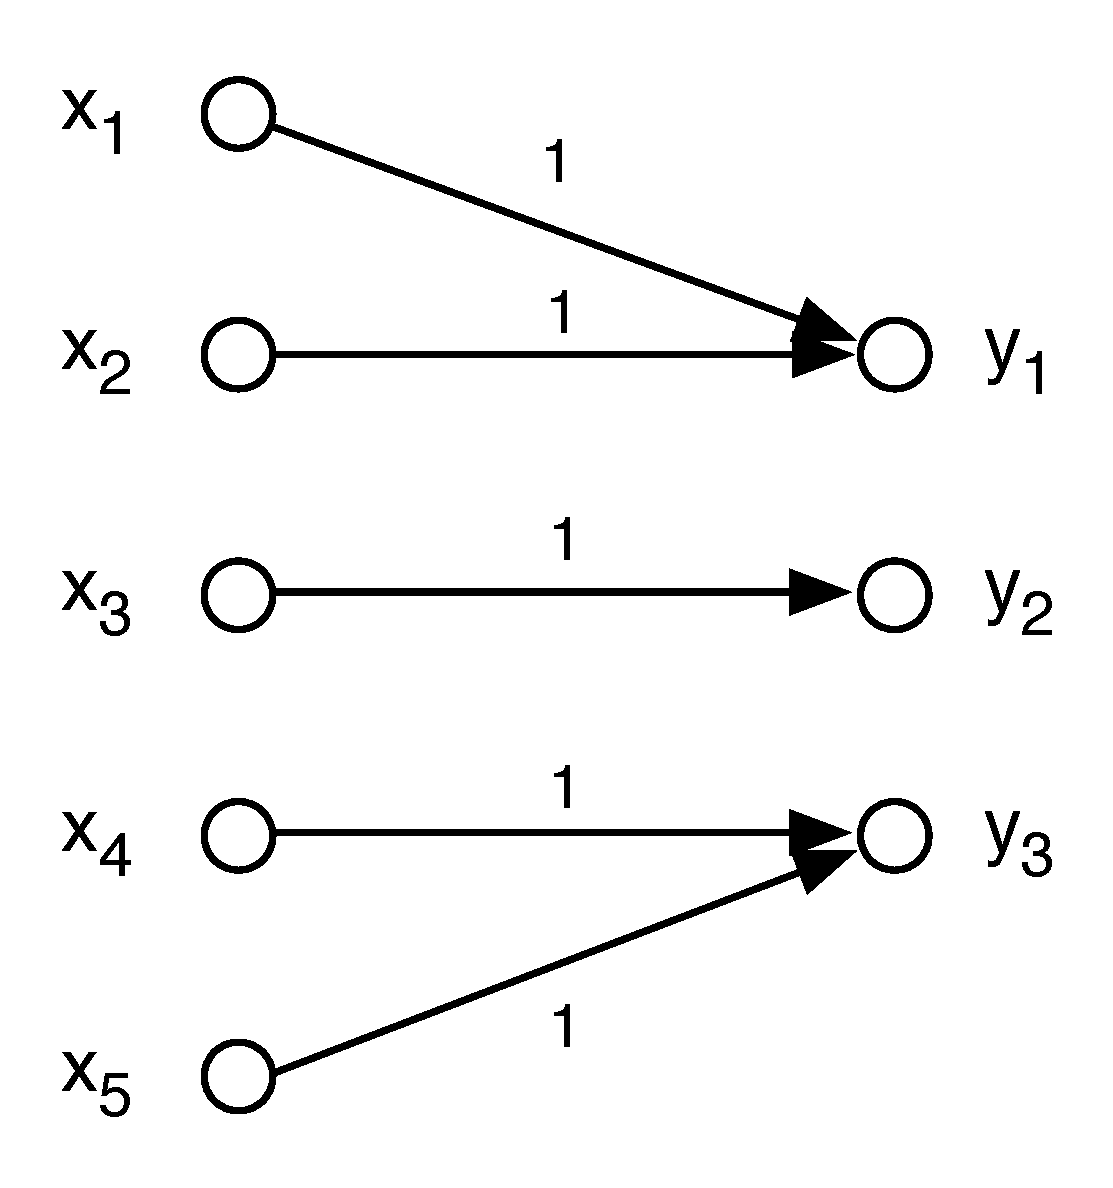
\includegraphics[width=0.4\textwidth]{img/determ1.pdf}}        
  \hspace{1cm}
  \subfloat[Matrice di canale]{\label{fig:determ2}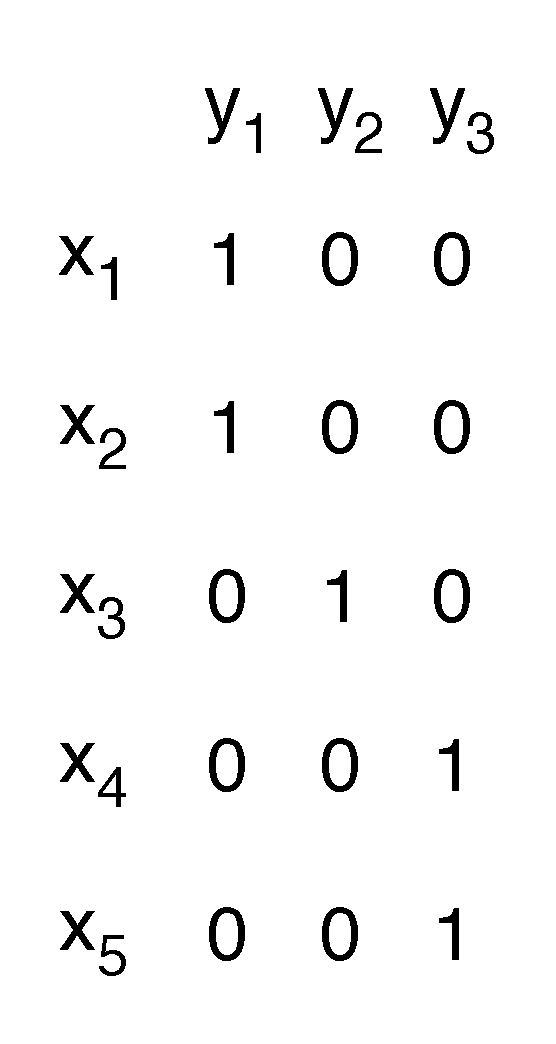
\includegraphics[width=0.25\textwidth]{img/determ2.pdf}}
  \caption{Esempio di canale deterministico}
  \label{fig:deterministico}
\end{figure}

\begin{lemma}
 Se $\C$ è deterministico, allora $H(Y/X)=0$
 \begin{proof}
  \[
   H(Y/X)=\sum_{x \in X} p(x)H(Y/X=x)
  \]
  Ma $\forall x \in X$, H(Y/X=x)=0. Infatti:
  \[
   H(Y/X=x)=\sum_{y \in Y}p(y/x) log(p(y/x))
  \]
  E per la definizione di canale deterministico $p(y/x)=0 \lor p(y/x)=1$
 \end{proof}
\end{lemma}

Calcoliamo ora la capacità per un canale deterministico.

\begin{lemma}
Se $\C$ è deterministico, allora $C=log|Y|$
\begin{proof}
 \[
  C=\max_{p(x)} I(X;Y)=\max_{p(x)} H(Y)-H(Y/X)
 \]
 Ora per il lemma precedente H(Y/X) è 0, da cui:
 \[
  C=\max_{p(x)} H(X)-H(X/Y)=\max_{p(x)} H(Y)
 \]
 Analogamente al canale noiseless, si ha il massimo che è pari al logaritmo, con distribuzione uniforme:
 \[
  C=\max_{p(x)} H(Y)=log|Y|
 \]
 Tuttavia questa volta la distribuzione uniforme deve essere $p(y)$!
 L'ultima considerazione è dunque valida se esiste una distribuzione $p(x)$, tale che $p(y)$ sia uniforme.
 Poniamo:
 \[
  X(y)=\{x \in X \ / \ p(y/x)=1 \}
 \]
 Allora la distribuzione $p(x)$ che rende uniforme $p(y)$ è:
 \[
  p(x)=\frac{1}{|Y| \ |X(y)|}
 \]
 Ciò è vero in quanto:
 \[\begin{split}
  p(y)&=\sum_{x \in X}p(x)p(y/x) \\
      &=\sum_{x \in X(y)}p(x) \\
      &=\sum_{x \in X(y)}\frac{1}{|Y| \ |X(y)|} \\
      &=\frac{1}{|Y|} \frac{|X(y)|}{|X(y)|} \\
      &=\frac{1}{|Y|}
   \end{split}
 \]

\end{proof}
\end{lemma}


\subsection{Canale completamente deterministico}

\medskip

\begin{definizione}
 Un canale si dice completamente deterministico (uno a uno) se è noiseless e deterministico.
\end{definizione}

In questo caso quindi sia il mittente che il destinatario sanno cosa è stato ricevuto/inviato.
In figura \ref{fig:cdeterministico} è riportato un esempio di canale completamente deterministico.

\begin{figure}[htbp]
  \centering
  \subfloat[Grafo di canale]{\label{fig:cdeterm1}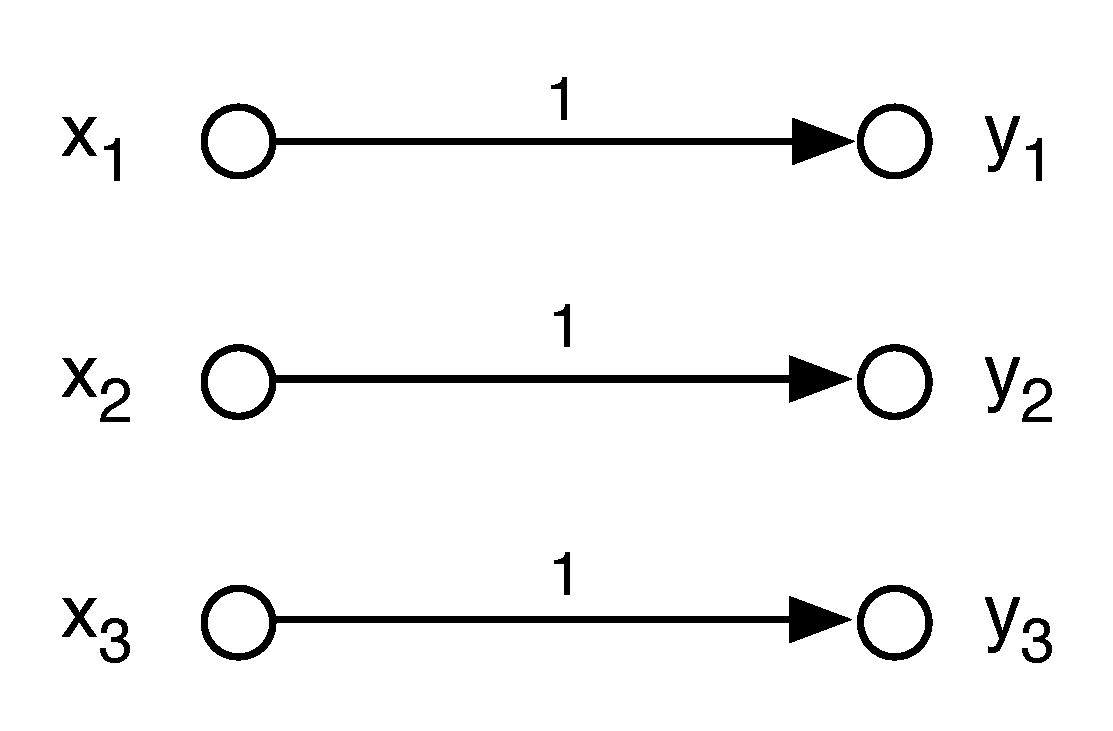
\includegraphics[width=0.4\textwidth]{img/cdeterm1.pdf}}        
  \hspace{1cm}
  \subfloat[Matrice di canale]{\label{fig:cdeterm2}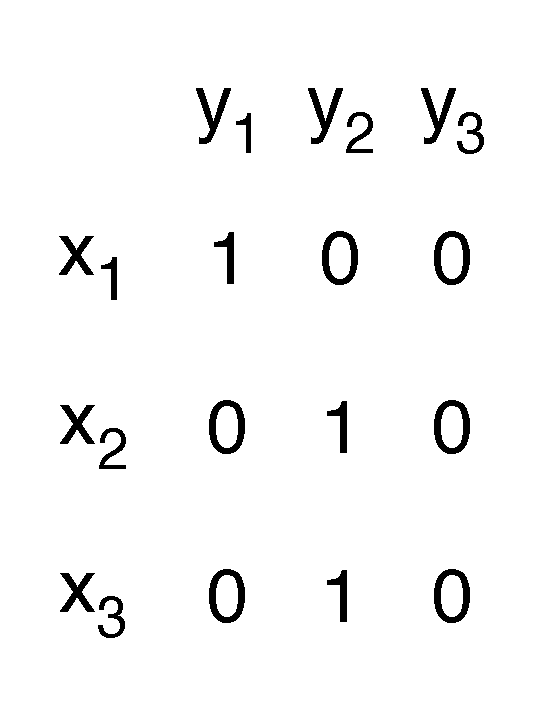
\includegraphics[width=0.25\textwidth]{img/cdeterm2.pdf}}
  \caption{Esempio di canale completamente deterministico}
  \label{fig:cdeterministico}
\end{figure}

\begin{lemma}
 Se $\C$ è completamente completamente deterministico, allora:
 \begin{itemize}
  \item $H(Y/X)=H(X/Y)=0$
  \item $I(X;Y)=H(X)=H(Y)$
 \end{itemize}
 \begin{proof}
  Il primo punto segue direttamente dai lemmi per il canale noiseless e deterministico.
  Il secondo punto è la solita proprietà dell'informazione mutua:
  \[\begin{split}
   I(X;Y)&=H(X)-H(X/Y)=H(X) \\
   I(X;Y)&=H(Y)-H(Y/X)=H(Y)
   \end{split}
  \]

 \end{proof}
\end{lemma}

\noindent
Per quanto riguarda infine la capacità di canale:

\begin{lemma}
Se $\C$ è completamente deterministico, allora $C=log|X|=log|Y|$
\begin{proof}
Segue direttamente dai lemmi per il canale noiseless e deterministico.
\end{proof}
\end{lemma}



\subsection{Canale inutile}

\medskip

\begin{definizione}
 Un canale si dice inutile (molti a molti) se:
 \[
  \forall y \in Y \ \exists C(y) \in R \ : \ \forall x \in X p(y/x)=C(y)
 \]
 Dove $C(y)$ è una costante che dipende da $y$.
\end{definizione}

In questo caso quindi le colonne della matrice di canale sono costanti, quindi le righe sono tutte identiche fra loro.
In figura \ref{fig:inutile} è riportato un esempio di canale inutile. Osservando il grafo di canale (o la matrice) è facile capire
come mai il canale è detto ``inutile''. Infatti il mittente ed il destinatario non potranno derivare alcuna informazione dalla 
comunicazione...che è stata appunto inutile.

\begin{figure}[htbp]
  \centering
  \subfloat[Grafo di canale]{\label{fig:inutile1}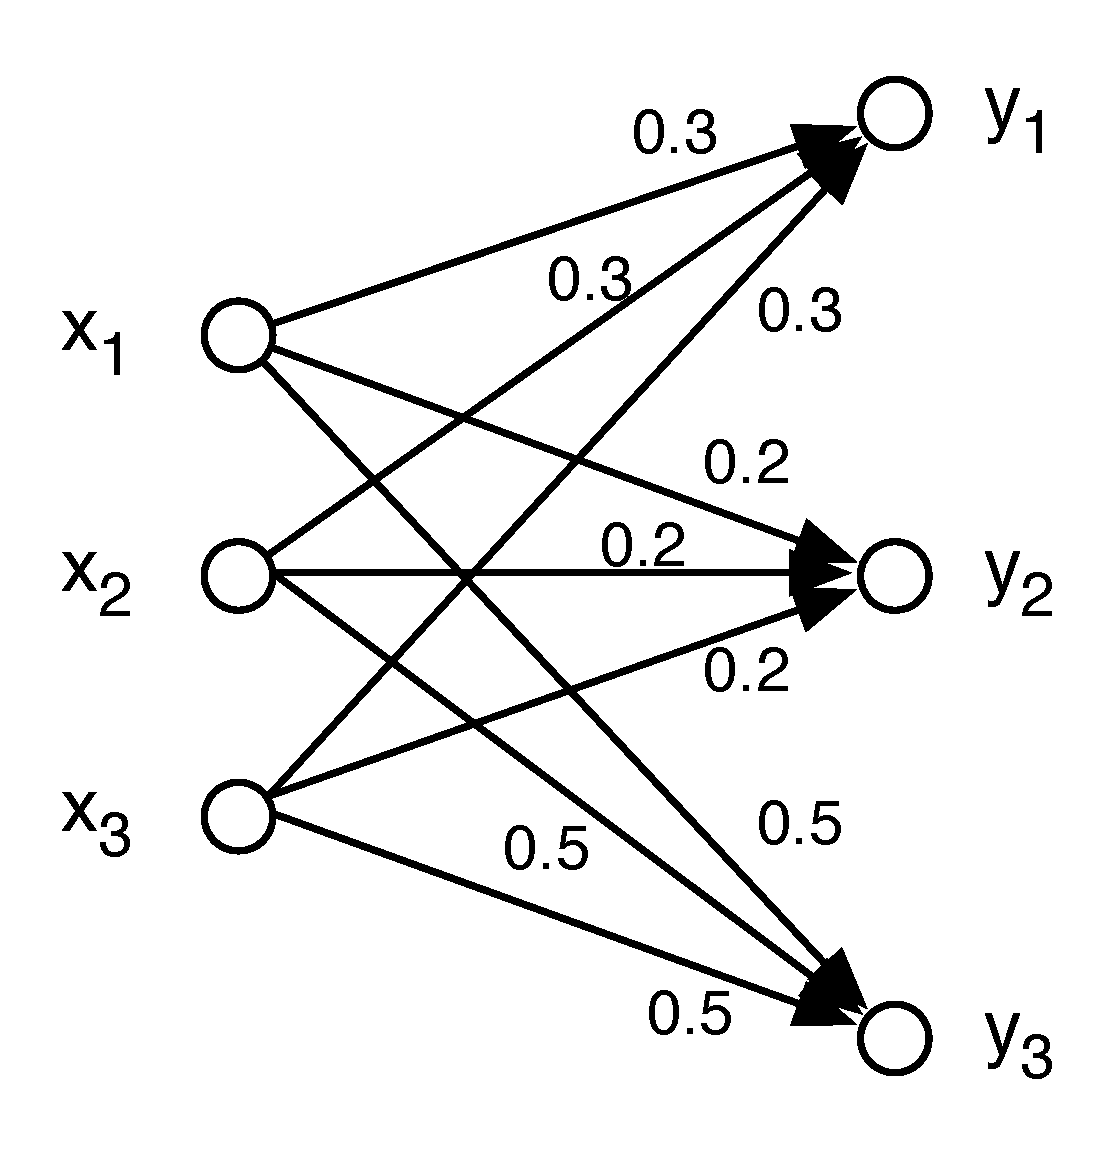
\includegraphics[width=0.5\textwidth]{img/inutile1.pdf}}        
  \hspace{1cm}
  \subfloat[Matrice di canale]{\label{fig:inutile2}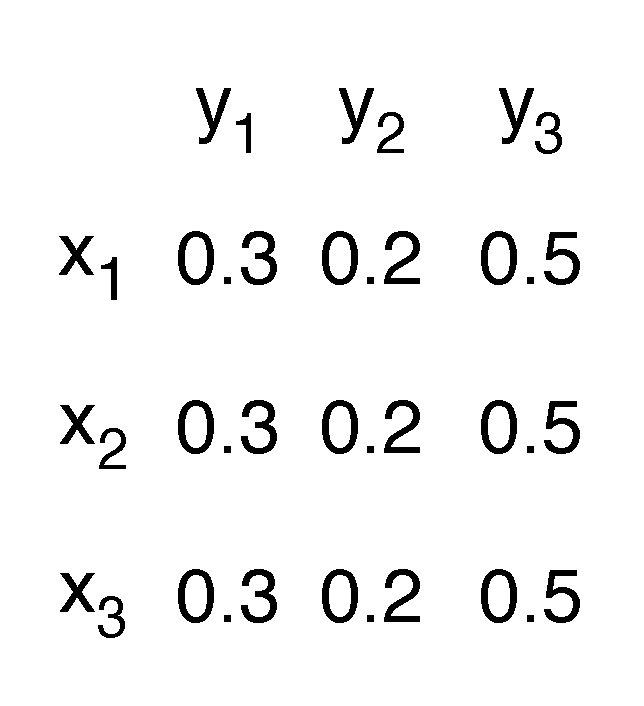
\includegraphics[width=0.25\textwidth]{img/inutile2.pdf}}
  \caption{Esempio di canale inutile}
  \label{fig:inutile}
\end{figure}

\begin{lemma}
 Se $\C$ è inutile, allora:
\[
  I(X;Y)=0
\]
 \begin{proof}
\[\begin{split}
 p(x,y)&=p(x)p(y/x) \\
       &=p(x)p(y/x)\sum_{x \in X}p(x) 
       =p(x)C(y)\sum_{x \in X}p(x) \\
       &=p(x) \sum_{x \in X}p(x)C(y)
       =p(x) \sum_{x \in X}p(x)p(y/x)\\
       &=p(x) p(y) \\
  \end{split}
\]
Quindi $p(x,y)=p(x)p(y)$, il che implica che $X$ e $Y$ sono indipendenti.
Ma se $X$ e $Y$ sono indipendenti, per l'osservazione \ref{mutuaindip} si ha $I(X;Y)=0$
 \end{proof}
\end{lemma}

\noindent
Per quanto riguarda infine la capacità di canale:

\begin{lemma}
Se $\C$ è inutile, allora $C=0$
\begin{proof}
Segue direttamente dal lemma precedente.
\end{proof}
\end{lemma}

\subsection{Canale simmetrico}

\medskip

\begin{definizione}
 Un canale si dice simmetrico se:
 \begin{enumerate}
  \item Le righe nella sua matrice di canale sono uguali a meno di una permutazione
  \item Le colonne nella sua matrice di canale sono uguali a meno di una permutazione
 \end{enumerate}
\end{definizione}


\begin{table}[htbp]
  \begin{center}
   \begin{tabular}{c c c c}
	& $y_1$ & $y_2$ & $y_3$ \\
	$x_1$ & 0.3 & 0.2 & 0.5 \\ 
	$x_2$ & 0.5 & 0.3 & 0.2  \\ 
	$x_3$ & 0.2 & 0.5 & 0.3  \\ 
    \end{tabular}
  \caption{Esempio di canale simmetrico (Matrice di canale).}
  \label{tab:tsim}
  \end{center}
\end{table}

\begin{lemma}
 Se $\C$ è un canale simmetrico, c una riga ed r una colonna della sua matrice di canale, allora:
 \begin{enumerate}
  \item $H(Y/X)=H(r)$
  \item $H(X/Y)=H(c)$
 \end{enumerate}
 \begin{proof}
  \mbox{}

  \noindent
  Per quanto riguarda il primo punto:
  \[
   H(Y/X)=\sum_{x \in X}p(x)H(Y/X=x)
  \]
  Ma le righe sono tutte uguali a meno di una permutazione, quindi H(Y/X=x) è costante, da cui:
  \[
   H(Y/X)=H(r)\sum_{x \in X}p(x)=H(r)
  \]
  Il secondo punto è del tutto analogo, visto che anche le colonne sono uguali a meno di una permutazione.
 \end{proof}

\end{lemma}

\noindent
Un esempio di canale simmetrico è riportato in tabella \ref{tab:tsim}.
La capacità di un canale simmetrico è fornita dal seguente teorema

\begin{teorema}
 Se $\C$ è un canale simmetrico ed r una riga della matrice di canale di $\C$, allora:
 \[
  C=log|Y| - H(r)
 \]
 \begin{proof}
\[
  C=\max_{p(x)} I(X;Y)=\max_{p(x)} H(Y)-H(Y/X)
\]
 Ora per il lemma precedente:
 \[
  \max_{p(x)} H(Y)-H(Y/X)=\max_{p(x)} H(Y)-H(r)
 \]
 H(r) non dipende da p(x), quindi basta massimizzare H(Y) che come già visto ha massimo in $log|Y|$. Quindi:
 \[
  C=\max_{p(x)} H(Y)-H(r)=log |Y| - H(r)
 \]
 Il risultato si ottiene, come già visto per il canale deterministico, quando $p(y)$ ha distribuzione uniforme.
 Tuttavia in questo caso anche $p(x)$ deve essere uniforme. Infatti:
 \[
  p(x)=\frac{1}{|X|} \Rightarrow p(y)=\frac{1}{|Y|}
 \]
 Ciò si ricava facilmente da:
 \[
  p(y)=\sum_{x \in X} p(x)p(y/x)=\frac{1}{|X|} \sum_{x \in X}p(y/x)
 \]
 Ma la somma degli elementi di ogni colonna è costante, quindi:
 \[
  \frac{1}{|X|} \sum_{x \in X}p(y/x)=\frac{1}{|X|} const=\frac{1}{|Y|}
 \]
 \end{proof}

\end{teorema}

\subsection{Canale debolmente simmetrico}

\medskip

\begin{definizione}
 Un canale si dice debolmente simmetrico se:
 \begin{enumerate}
  \item Le righe nella sua matrice di canale sono uguali a meno di una permutazione
  \item La somma degli elementi di ciascuna colonna nella sua matrice di canale è costante
 \end{enumerate}
\end{definizione}

\begin{table}[htbp]
  \begin{center}
   \begin{tabular}{c c c c}
	  & $y_1$ & $y_2$ & $y_3$ \\
	$x_1$ & 1/3 & 1/6 & 1/2 \\ 
	$x_2$ & 1/3 & 1/2 & 1/6  \\ 
    \end{tabular}
  \end{center}
  \label{tdsim}
  \caption{Esempio di canale debolmente simmetrico (Matrice di canale).}
\end{table}

\noindent
Un esempio di canale debolmente simmetrico è riportato in tabella \ref{tdsim}.
La capacità di canale è uguale a quella dei canali simmetrici, come descritto dal seguente teorema.

\begin{teorema}
 Se $\C$ è un canale debolmente simmetrico ed $r$ una riga della matrice di canale di $\C$, allora:
 \[
  C=log|Y| - H(r)
 \]
 Il risultato si ottiene quando p(x) è uniforme.
\begin{proof}
 E' esattamente identica a quella del canale simmetrico.
\end{proof}

\end{teorema}

\subsection{Binary Symmetric Channel}

Il Binary Symmetric Channel (BSC) è un particolare canale simmetrico composto da due simboli in ingresso e da due simboli in uscita (ne avevamo già visto un esempio in introduzione, figura \ref{fig:bsc}).

\begin{figure}[htbp]
  \centering
  \subfloat[Grafo di canale]{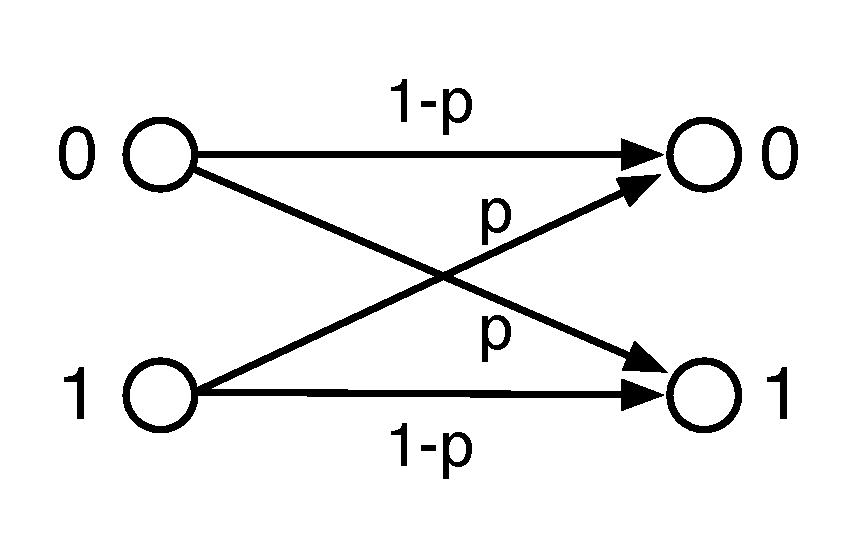
\includegraphics[width=0.4\textwidth]{img/bsc1.pdf}}        
  \hspace{1cm}
  \subfloat[Matrice di canale]{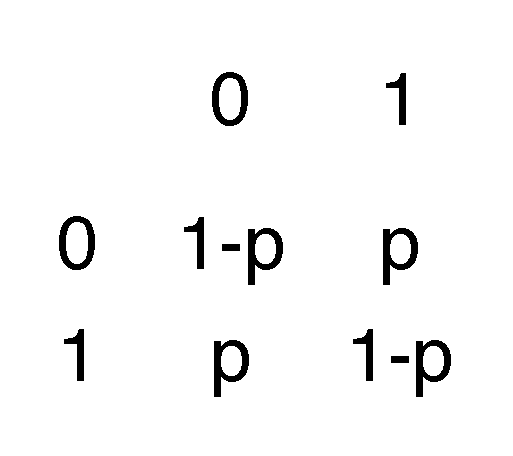
\includegraphics[width=0.25\textwidth]{img/bsc2.pdf}}
  \caption{BSC}
  \label{fig:bsc2}
\end{figure}

Il canale è rappresentato in figura \ref{fig:bsc2}. Con p abbiamo quindi indicato la probabilità che ci sia un errore di trasmissione.
Siamo ora interessati a calcolare la capacità di questo canale.
Innanzitutto indichiamo con $\Pi$ la probabilità che la sorgente emetta il simbolo 0, ovvero:
\[
 \Pi=P\{X=0\}
\]
Calcoliamo ora l'informazione mutua:
\[
 I(X;Y)=H(Y)-H(Y/X)
\]
Calcoliamo il primo termine. In questo caso la variabile $Y$ ha due simboli, quindi l'entropia 
sarebbe formata da due elementi ($Y=0$ e $Y=1$), tuttavia ne indichiamo solo uno $(Y=1)$. L'altro infatti si può ricavare 
al solito come differenza, tenendo conto che la somma è 1. 
\[
 H(Y)=H(\Pi p + (1-\Pi)(1-p))
\]
Per il secondo termine:
\[\begin{split}
 H(Y/X)&=\Pi H(Y/X=0) + (1-\Pi) H(Y/X=1) \\
       &=\Pi H(p) + (1-\Pi) H(p) \\
       &=H(p)
  \end{split}
\]
A questo punto la capacità di canale è:
\[
 C=\max_{p(x)} I(X;Y)=\max_{0 \le \Pi \le 1} I(X;Y)=\max_{0 \le \Pi \le 1} [ H(\Pi p + (1-\Pi)(1-p)) - H(p) ]
\]
Dobbiamo ora trovare il valore di $\Pi$ che massimizza l'informazione mutua, ovvero:
\[
 arg \max_{0 \le \Pi \le 1} [ H(\Pi p + (1-\Pi)(1-p)) - H(p) ]
\]
Ma H(p) non dipende da $\Pi$, quindi basta risolvere:
\[
 arg \max_{0 \le \Pi \le 1} [ H(\Pi p + (1-\Pi)(1-p))]
\]
Ma sappiamo che l'entropia raggiunge il massimo quando le componenti sono equiprobabili.
In questo caso abbiamo due componenti, quindi deve essere:
\[\begin{split}
 &\Pi p + (1-\Pi)(1-p)=\frac{1}{2} \\
 \Rightarrow &\Pi p + 1-p + -\Pi +\Pi p=\frac{1}{2} \\ 
 \Rightarrow &\Pi(2p-1) + 1-p =\frac{1}{2} \\ 
 \Rightarrow &\Pi(2p-1) =\frac{1}{2}-1+p \\ 
 \Rightarrow &\Pi(2p-1) =-\frac{1}{2}+p \\
 \Rightarrow &\Pi=\frac{-\frac{1}{2}+p}{2p-1} \\  
 \Rightarrow &\Pi=\frac{p-\frac{1}{2}}{2(p-\frac{1}{2})} \\
 \Rightarrow &\Pi=\frac{1}{2} \\
  \end{split}
\]

\noindent
Dunque si ha il massimo quando $\Pi=1/2$, ovveroquando la sorgente emette in maniera equiprobabile 0 o 1.
Infine, poiche $H(1/2,1/2)=1$, la capacità di canale di un BSC è:

\[
 C=1-H(p)
\]

In figura \ref{fig:cbsc} è rappresentata la capacità del canale, al variare di p.
Come si nota quando $p=0$ (o $p=1$) la capacità è massima, infatti sul canale circola un grande contenuto informativo, non c'è infatti 
alcuna incertezza. Viceversa quando $p=1/2$ sul canale non viaggia alcuna informazione. Il destinatario infatti alla ricezione di un simbolo non è in grado di inferire nulla (in questo caso si ha un canale inutile).

\begin{figure}[htbp]
\begin{center}
	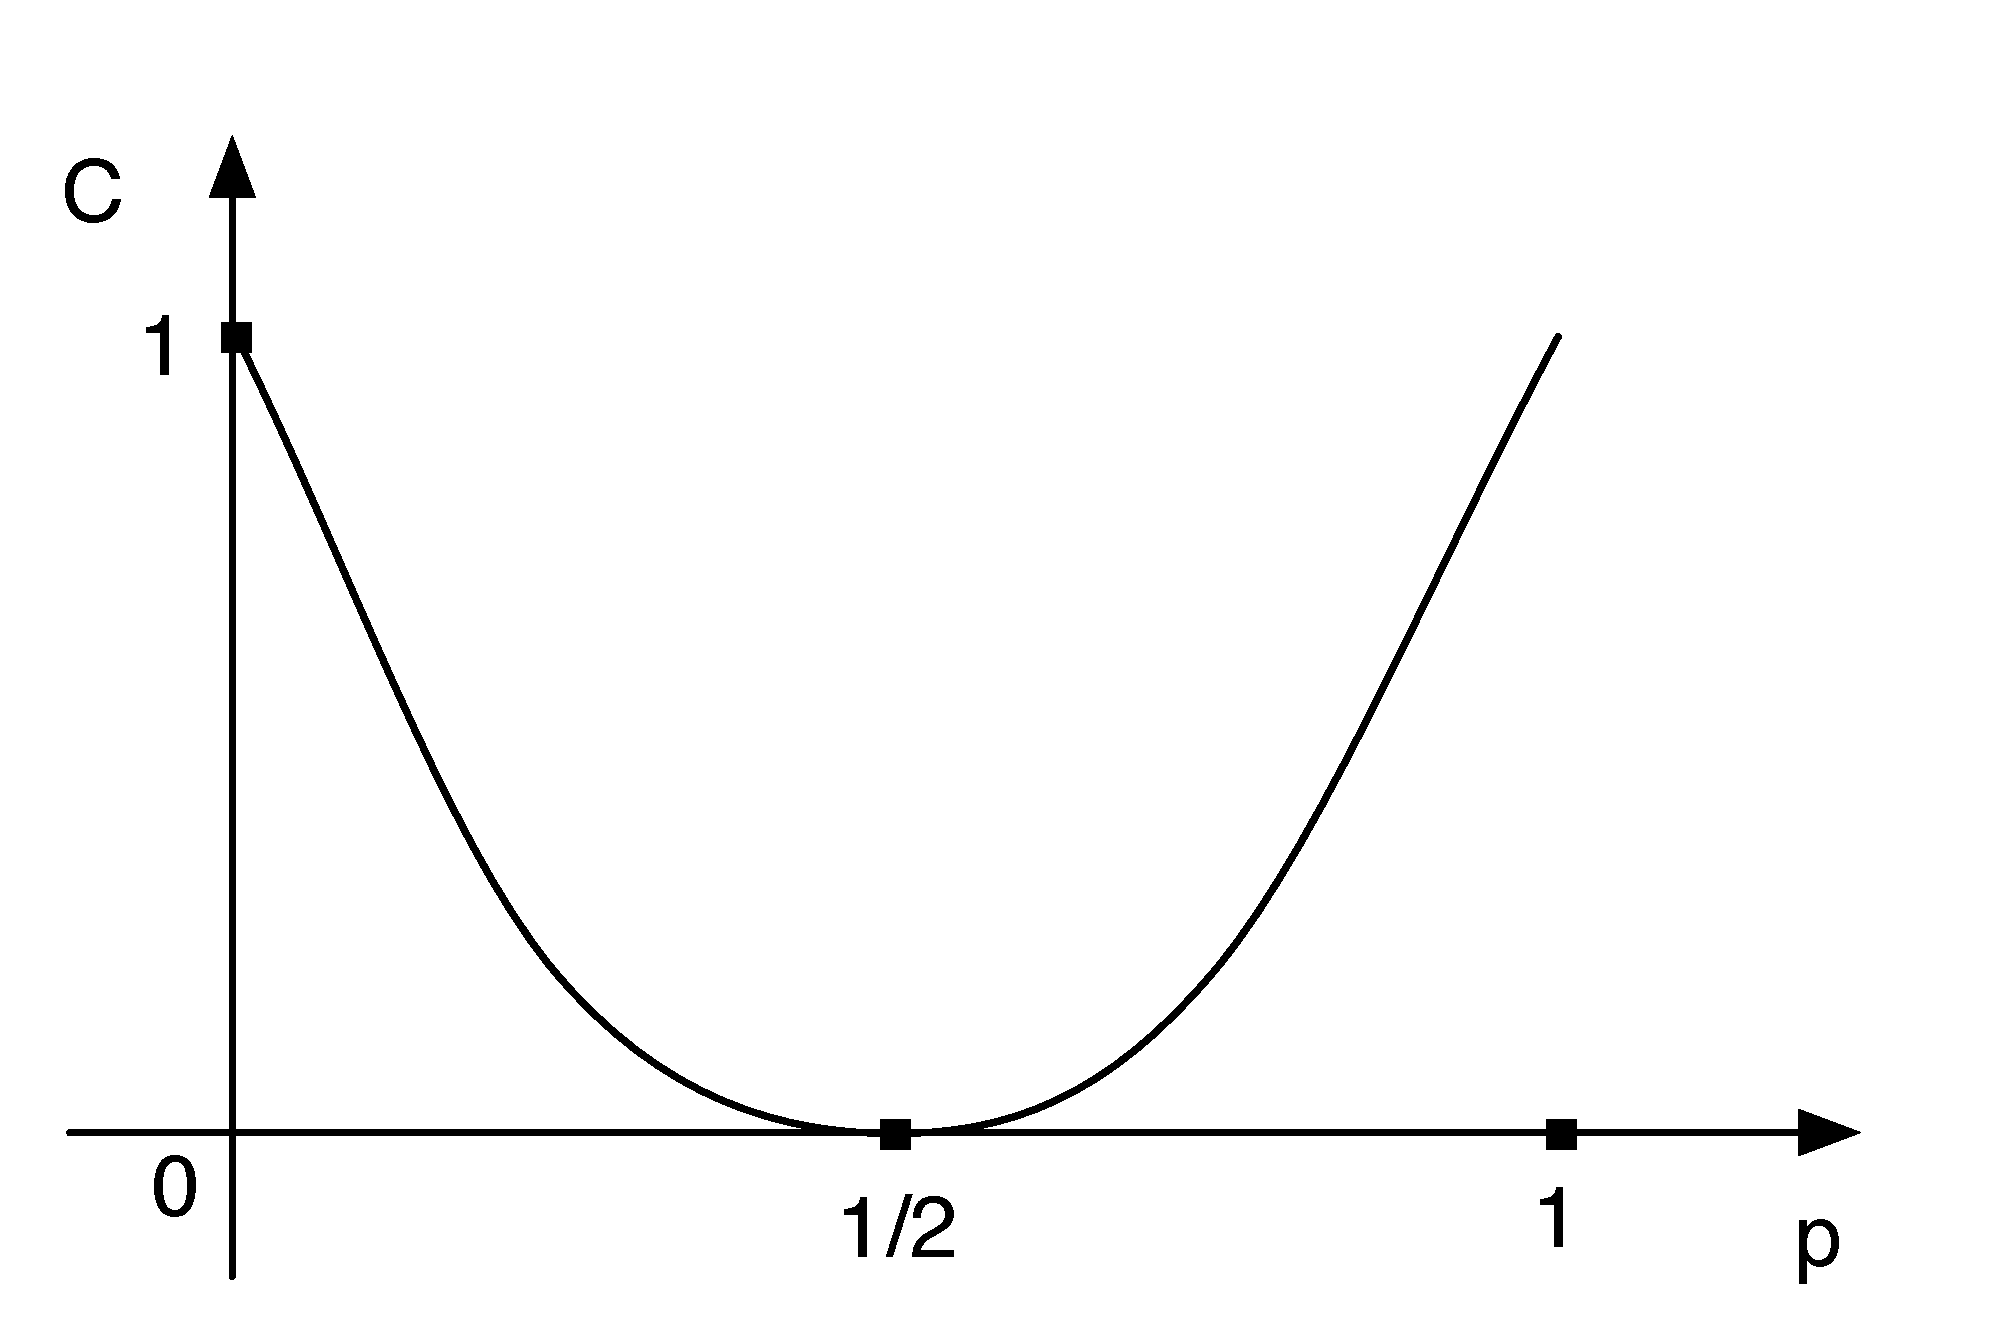
\includegraphics[width=0.6\textwidth]{img/cbsc.pdf}
\caption{Capacità di canale di un BSC al variare di p}
\label{fig:cbsc}
\end{center}
\end{figure}

\newpage

\subsection{Binary Erasure Channel}
Nel Binary Erasure Channel (BEC), il mittente può inviare due diversi simboli al destinatario. Un simbolo può essere ricevuto 
correttamente oppure ``perso'' (in questo caso il destinatario riceve uno speciale simbolo $\sharp$). Il canale ha dunque 2 ingressi, 3 uscite 
ed un parametro p che indica la probabilità di ``perdere'' il simbolo. Il canale è rappresentato in figura \ref{fig:bec}.

\begin{figure}[htbp]
  \centering
  \subfloat[Grafo di canale]{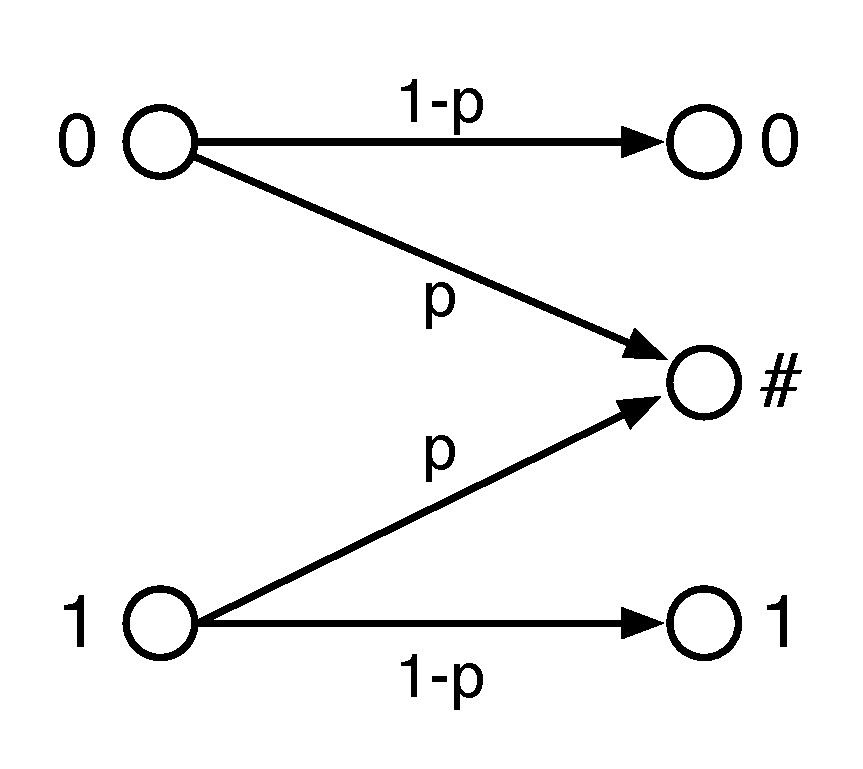
\includegraphics[width=0.35\textwidth]{img/bec1.pdf}}        
  \hspace{1cm}
  \subfloat[Matrice di canale]{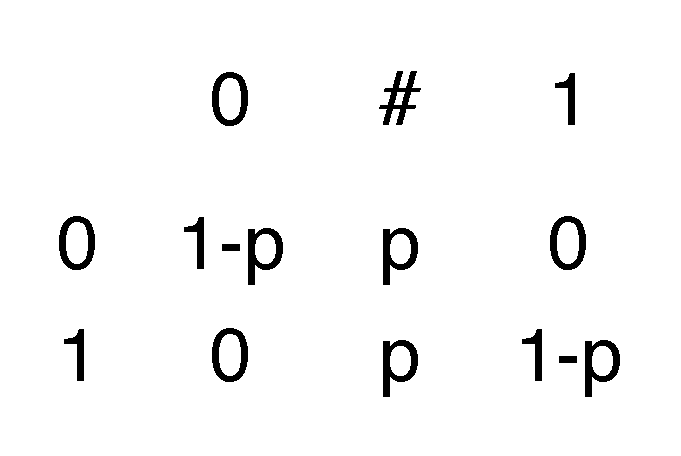
\includegraphics[width=0.26\textwidth]{img/bec2.pdf}}
  \caption{BEC}
  \label{fig:bec}
\end{figure}

\noindent
Procediamo al calcolo della capacità di canale. Come per il BSC poniamo:
\[
 \Pi=P\{X=0\}
\]
Ora per calcolare l'informazione mutua ricaviamo:
\[
 H(Y)=H(Y=0,Y=1,Y=\sharp)=H(\Pi (1-p), (1-\Pi) (1-p), p)
\]
E:
\[\begin{split}
 H(Y/X)&=\Pi H(Y/X=0) + (1-\Pi) H(Y/X=1) \\
       &=\Pi H(1-p,p,0) + (1-\Pi) H(0,p,1-p) \\
       &=\Pi H(p) + (1-\Pi) H(p) \\
       &=H(p)
  \end{split}
\]
Quindi:
\[
 I(X;Y)=H(Y)-H(Y/X)=H(\Pi (1-p), (1-\Pi) (1-p), p) - H(p)
\]
La capacità di canale è dunque:
\[
 C=\max_{0 \le \Pi \le 1} H(\Pi (1-p), (1-\Pi) (1-p), p) - H(p)
\]
In maniera analoga al BSC, $H(p)$ non dipende da $\Pi$, quindi per massimizzare 
l'informazione mutua bisogna massimizzare la prima entropia.
Ma sappiamo che la funzione entropia è continua e concava (oss. \ref{entrconcava}).
Quindi esiste un solo massimo, quando la derivata è 0. Calcoliamo allora la derivata
(poniamo per brevità $q=1-p$):

\[\begin{split}
 &\frac{d}{d \Pi}  H(\Pi (1-p), (1-\Pi) (1-p), p) \\
 =&\frac{d}{d \Pi} H(\Pi q, (1-\Pi) q, p) \\
 =&\frac{d}{d \Pi} - [ \ \Pi q log(\Pi q) + (1-\Pi) q log((1-\Pi)q) + plog(p) \ ] \\
 =&-[\Pi q \frac{1}{\Pi q} q + q log(\Pi q) + (1-\Pi)q \frac{1}{(1-\Pi)q} (-q) + -qlog((1-\Pi)q) ] \\
 =&-[q + q log(\Pi q) -q -qlog((1-\Pi)q) ] \\
 =&-q[log(\Pi q) -log((1-\Pi)q) ] \\
 =&-qlog \frac{\Pi q}{(1-\Pi)q}=-qlog \frac{\Pi}{1-\Pi}
  \end{split}
\]
Ora eguagliamo la derivata a 0 e ricaviamo $\Pi$:
\[\begin{split}
 &-qlog \frac{\Pi}{1-\Pi}=0 \\
 \Rightarrow &\frac{\Pi}{1-\Pi}=1 \\
 \Rightarrow &\Pi=1-\Pi \\
\Rightarrow &\Pi=\frac{1}{2}
  \end{split}
\]
Quindi si ha il massimo quando $\Pi=\frac{1}{2}$.
La capacità di canale è dunque (si ponga sempre attenzione al fatto che come al solito $H(p)=H(p,1-p)$ ):
\[\begin{split}
C=&H(\frac{1}{2} q, \frac{1}{2} q, p) - H(p) \\
=& -\frac{q}{2} log\frac{q}{2} - \frac{q}{2} log\frac{q}{2}  - plog(p) +p log(p) +q log(q)\\
=&-qlog\frac{q}{2}+q log(q)  \\
=&qlog(2) -qlog(q) +q log(q)\\
=&qlog(2) \\
=&q=1-p
\end{split}
\]

\subsection{Canale Z}
Il canale Z è composto da 2 simboli. Un simbolo arriva con certezza in maniera corretta al destinatario, mentre l'altro può essere 
tramutato nel primo con probabilità (quindi di errore) $p$. Il canale è rappresentato in figura \ref{fig:z}.

\begin{figure}[htbp]
  \centering
  \subfloat[Grafo di canale]{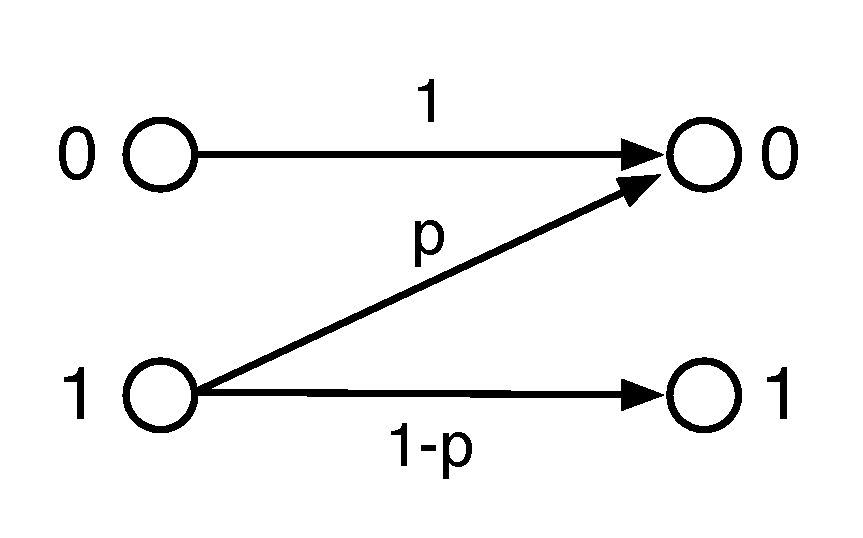
\includegraphics[width=0.35\textwidth]{img/z1.pdf}}        
  \hspace{1cm}
  \subfloat[Matrice di canale]{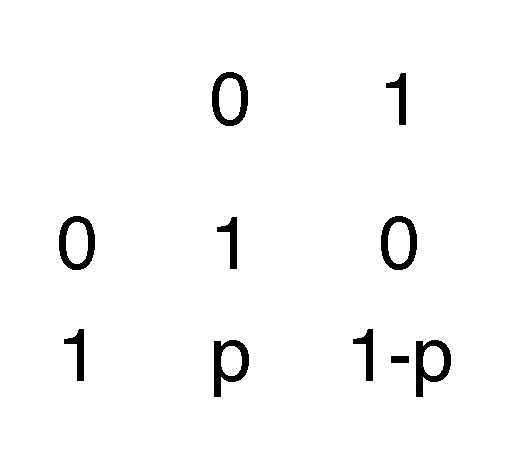
\includegraphics[width=0.26\textwidth]{img/z2.pdf}}
  \caption{Canale Z}
  \label{fig:z}
\end{figure}

\noindent
Calcoliamo ora la capacità del canale Z.
Poniamo (diversamente da prima!):
\[
 \Pi=P\{X=1\}
\]
Ora per calcolare l'informazione mutua ricaviamo:
\[\begin{split}
 H(Y)=&H(1-\Pi+\Pi p,\Pi (1-p)) \\
     =&H(1-\Pi(1-p),\Pi(1-p)) \\
     =&H(\Pi(1-p))
  \end{split}
\]
E:
\[\begin{split}
 H(Y/X)=&\Pi H(Y/X=1)+(1-\Pi)H(Y/X=0) \\
     =&\Pi H(p) + (1-\Pi)H(1) \\
     =&\Pi H(p) 
  \end{split}
\]
L'informazione mutua è dunque:
\[
 I(X;Y)=H(Y)-H(Y/X)=H(\Pi(1-p))-\Pi H(p)
\]
Al solito, per trovare la capacità del canale dobbiamo trovare il massimo 
dell'informazione mutua al variare di $\Pi$.
Per le stesse considerazione del BEC, vediamo dove la derivata si annulla.
Calcoliamo quindi la derivata dell'informazione mutua (per comodità $q=1-p$):
\[\begin{split}
 &\frac{d}{d \Pi}  H(\Pi(1-p))-\Pi H(p) \\
 =&\frac{d}{d \Pi}  H(\Pi q)-\Pi H(p) \\
 =&\frac{d}{d \Pi} -\Pi q log(\Pi q) - (1-\Pi q) log(1-\Pi q) -\Pi H(p) \\
 =& -\Pi q \frac{1}{\Pi q} q - qlog(\Pi q)  + \\
  &  -(1-\Pi q) \frac{1}{1-\Pi q} (-q) + q log(1- \Pi q)   +  \\
  &  -H(p) \\
 =& -q -qlog(\Pi q)+ q + qlog(1-\Pi q) -H(p) \\
 =& qlog \frac{1-\Pi q}{\Pi q} -H(p)
 \end{split}
\]
Ora equagliamo la derivata a 0 e ricaviamo $\Pi$:
\[\begin{split}
 & qlog \frac{1-\Pi q}{\Pi q} - H(p)=0 \\
 \Rightarrow & qlog \frac{1-\Pi q}{\Pi q}=H(p) \\
 \Rightarrow & log \frac{1-\Pi q}{\Pi q}=\frac{H(p)}{q} \\
 \Rightarrow & \frac{1-\Pi q}{\Pi q}=2^{\frac{H(p)}{q}} \\
 \Rightarrow & \frac{1}{\Pi q}-1=2^{\frac{H(p)}{q}} \\
 \Rightarrow & \frac{1}{\Pi q}=2^{\frac{H(p)}{q}}+1 \\
 \Rightarrow & \Pi=\frac{1}{q(2^{\frac{H(p)}{q}}+1)}
\end{split}
\]
Ora possiamo concludere calcolando la capacità del canale:
\[\begin{split}
 C=& H \left ( \frac{q}{q(2^{\frac{H(p)}{q}}+1)} \right)-\frac{1}{q(2^{\frac{H(p)}{q}}+1)} H(p) \\
  =& H \left (\frac{1}{2^{\frac{H(p)}{q}}+1} \right)-\frac{1}{q(2^{\frac{H(p)}{q}}+1)} H(p) \\
  =& H \left (\frac{1}{2^{\frac{H(p)}{q}}+1} \right)-\frac{H(p)}{q(2^{\frac{H(p)}{q}}+1)} \\
  =& H \left (\frac{1}{2^{\frac{H(q)}{q}}+1} \right)-\frac{H(q)}{q(2^{\frac{H(q)}{q}}+1)} \\
 \end{split}
\]


\section{Regole di decisione}
Sono state descritte varie tipologie di canale e soprattutto il concetto di capacità (di canale). Tuttavia, non abbiamo ancora chiarito 
il funzionamento della comunicazione in un canale rumoroso. Vediamo dunque in dettaglio come avviene la comunicazione.
Il mittente codifica il messaggio da inviare e manda quindi sul canale delle parole di codice (formate da simboli).
A partire dai simboli inviati, quelli che vengono ricevuti dipendono dal canale (come specificato dalla matrice o dal grafo di canale).
A questo punto il destinatario deve essere in grado di determinare le parole di codice inviate.
C'è bisogno in sostanza di una \textbf{regola di decisione}, che consenta di passare dai simboli ricevuti a quelli inviati.

\begin{definizione}
 Dato un canale $\mathcal{C}=(X,p(y/x),Y)$, una regola di decisione è una funzione
 \[
  d: Y \to X
 \]
\end{definizione}

\noindent
\textbf{Esempio}

\noindent
Data la seguente matrice di canale:

\begin{table}[htbp]
  \begin{center}
   \begin{tabular}{c c c c}
	& $y_1$ & $y_2$ & $y_3$ \\
	$x_1$ & 0.5 & 0.3 & 0.2 \\ 
	$x_2$ & 0.2 & 0.3 & 0.5  \\ 
	$x_3$ & 0.3 & 0.3 & 0.4  \\ 
    \end{tabular}
  \end{center}
\end{table}

\noindent
Una possibile regola di decisione è:
$d(y_1)=x_1$, 
$d(y_2)=x_2$, 
$d(y_3)=x_2$

\noindent
Un'altra possibile regola è:
$d(y_1)=x_1$, 
$d(y_2)=x_3$, 
$d(y_3)=x_2$

\noindent
Ancora, una terza regola può essere:
$d(y_1)=x_2$, 
$d(y_2)=x_2$, 
$d(y_3)=x_1$

\bigskip

Chiaramente una regola di decisione, dovrebbe cercare di ridurre l'errore al minimo. In pratica, dovrebbe essere tale da identificare 
correttamente il simbolo inviato nella maggior parte dei casi. Nell'esempio fatto poco prima, intuitivamente la 3° regola sembra sicuramente da scartare.
Definiamo ora la probabilità di errore, in maniera da trovare una regola che la minimizzi:
\begin{definizione}
 Dato un canale $\mathcal{C}=(X,p(y/x),Y)$ ed una regola di decisione d, la probabilità di errore di d è:
\[
 P_E(d)=\sum_{y \in Y} P(E/y)p(y)
\]
Dove P(E/y) indica la probabilità di decidere un simbolo errato quando si riceve y.
\end{definizione}
\noindent
Per minimizzare la probabilità di errore, dobbiamo avere d in modo che:
\[
 d^*=\arg \min_d P_E(d)=\arg \min_d \sum_{y \in Y} P(E/y)p(y)
\]
Ma la sommatoria è di termini positivi (ed indipendenti), quindi per minimizzarla è sufficiente minimizzare ogni termine.
Inoltre $p(y)$ non dipende da $d$. Quindi:
\[
 \forall y \in Y \ : \ d(y)=\arg \min_d P(E/y)
\]

\noindent
A questo punto si nota che $P(E/y)=1-P(d(y)/y)$. Infatti la probabilità di decidere un simbolo errato, è complementare a quella di deciderlo in maniera corretta.
Risulta quindi:
\[
 \forall y \in Y \ : \ d(y)=\arg \max_d P(d(y)/y)
\]

\noindent
Possiamo ora formulare una regola di decisione, che minimizzi la probabilità di errore.

\begin{definizione}[Regola dell'osservatore ideale (ROI)]
\[
 \forall y \in Y \ : \ d(y)=\arg \max_{x \in X} p(x/y)
\]
\end{definizione}

La regola ROI è abbastanza intuitiva. Si sceglie sempre il simbolo che ha la probabilità maggiore di essere stato inviato, 
dato un simbolo ricevuto. Questa quantità è proprio $p(x/y)$.
Sebbene la regola ROI minimizzi la probabilità di errore (e sia quindi ottima in questo senso), ha un grande svantaggio.
E' infatti necessario conoscere la matrice $P(x/y)$ e quindi $P(x)$. In altre parole, bisogna avere delle informazioni sulle 
probabilità di invio dei simboli da parte della sorgente. Spesso però queste informazioni non sono disponibili. E' quindi necessaria 
un'altra regola, che non abbia bisogno di questa informazione.

Non conoscere $P(x)$, è equivalente a supporre che $P(x)$ abbia una distribuzione uniforme. In questo caso la regola ROI si modificherebbe 
in questo modo:
\[
 \forall y \in Y \ : \ d(y)=\arg \max_{x \in X} p(x/y)=\arg \max_{x \in X} p(x)p(y/x)=\arg \max_{x \in X} p(y/x)
\]

Arriviamo quindi direttamente ad un'altra regola:
\begin{definizione}[Regola della massima verosimiglianza (RMV)]
\[
 \forall y \in Y \ : \ d(y)=\arg \max_{x \in X} p(y/x)
\]
\end{definizione}

Questa regola non è ottima (non minimizza quindi la probabilità di errore), però come detto ha il vantaggio di poter essere utilizzata
quando non è disponibile $P(x)$.

\noindent
Valutiamo ora meglio la probabilità di errore, in maniera da terminare da cosa dipende:
\[\begin{split}
 P_E&=\sum_{y \in Y} P(E/y)p(y) \\
    &=1-\sum_{y \in Y} P(d(y)/y)p(y) \\
    &=1-\sum_{y \in Y} P(d(y),y) \\
    &=\sum_{y \in Y}\sum_{x \in X} p(x,y) - \sum_{y \in Y} P(d(y),y) \\
    &=\sum_{y \in Y}\sum_{x \in X}^{x \neq d(y)} p(x,y) \\
    &=\sum_{y \in Y}\sum_{x \in X}^{x \neq d(y)} p(x)p(y/x) \\
 \end{split}
\]

Quindi la probabilità di errore per una data regola di decisione dipende dal canale e dalla sorgente.
Se non conosco la sorgente (i.e. non conosco $P(x)$) e la considero con una distribuzione uniforme risulta:

\begin{equation}
 \begin{split}
 P_E &=\sum_{y \in Y}\sum_{x \in X}^{x \neq d(y)} p(x)p(y/x) \\
     &=\frac{1}{n}\sum_{y \in Y}\sum_{x \in X}^{x \neq d(y)} p(y/x) \\
 \end{split}
\label{perr}
\end{equation}

\section{Codici di canale}
Il nostro obiettivo, come ricordato più volte, è realizzare una trasmissione il più possibile affidabile e veloce.
Abbiamo dato una misura per l'affidabilità, che è la probabilità di errore enunciata nel paragrafo precedente. La velocità invece 
si può misurare facilmente in base al numero di bit inviati. Proviamo innanzitutto a migliorare l'affidabilità della trasmissione.

\begin{figure}[htbp]
\begin{center}
	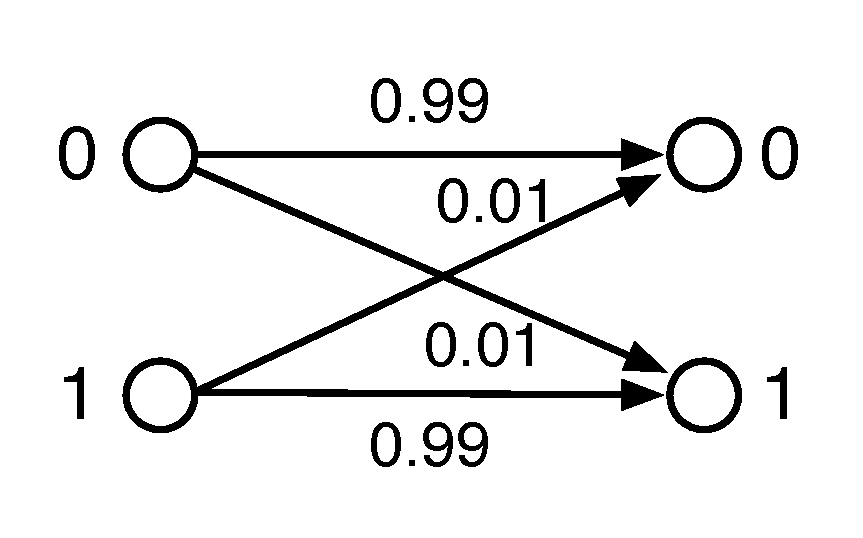
\includegraphics[width=0.4\textwidth]{img/bsc99.pdf}
\caption{BSC con p=0.01}
\label{fig:bsc99}
\end{center}
\end{figure}


Consideriamo un canale BSC con $p=0.01$ (figura \ref{fig:bsc99}) e supponiamo di non conoscere la sorgente, ovvero $P(x)$. La regola di decisione 
sarà dunque quella della massima verosimiglianza. Ovvero:
\[
 d(0)=0 \\ d(1)=1
\]
Calcoliamo quindi la probabilità di errore, con la formula \eqref{perr}:
\[
 P_E=\frac{0.01+0.01}{2}=0.01
\]

Proviamo ora a migliorare l'affidabilità. In maniera abbastanza banale, inseriamo un codificatore che invia 3 volte il bit (invece di una sola). In sostanza quindi stiamo considerando l'estensione terza di un BSC. La situazione è quella rappresentata in figura \ref{fig:bsc3}. I simboli che possono essere inviati sul canale sono solamente due (000 e 111), mentre possono essere ricevute tutte le 
combinazioni di 3 bit (a seguito degli errori di trasmissione).

\begin{figure}[htbp]
\begin{center}
	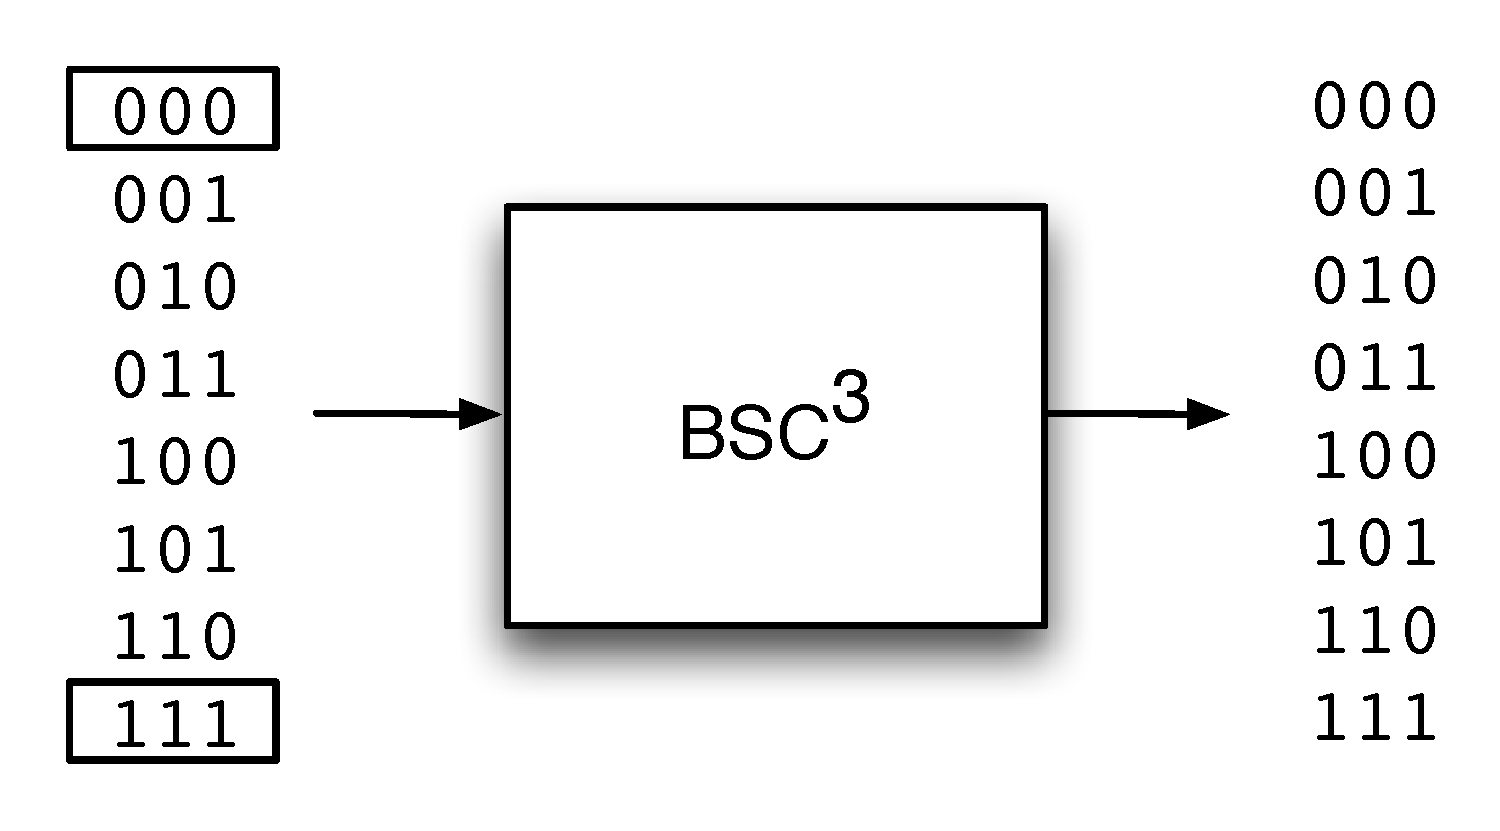
\includegraphics[width=0.6\textwidth]{img/bsc3.pdf}
\caption{$BSC^3$ con due possibili ingressi}
\label{fig:bsc3}
\end{center}
\end{figure}

La regola di decisione è abbastanza semplice. Si sceglie 0 se sono stati ricevuti più 0 che 1, mentre 1 nell'altro caso.
Poiché abbiamo scelto un'estensione dispari del canale, non ci troveremo mai nel caso in cui il numero di 0 e di 1 sia lo stesso.
Calcoliamo quindi la probabilità di errore in questo caso. Si ha un errore quando ci sono 2 o 3 bit errati. Se infatti è sbagliato 
un unico bit, si riesce banalmente a determinare il simbolo corretto. Quindi:
\[
 P_E=P(\sharp E=2)+P(\sharp E=3)
\]
Poiché la probabilità che un bit venga trasmesso in maniera non corretta è uguale a p=0.01 per tutti i simboli, si può utilizzare 
la distribuzione binomiale. Risulta quindi:
\[\begin{split}
 P_E&=p^2(1-p)^1 \binom{3}{2} + p^3(1-p)^0 \binom{3}{3} \\
    &=3p^2(1-p) +p^3 \\
    &=3 \cdot 0.01^2 \cdot 0.99 + 0.01^3 \\
    &\simeq 3 \cdot 10^{-4}
  \end{split}
\]
L'affidabilità è quindi aumentata rispetto al caso precedente. Tuttavia anche il numero di bit è aumentato, di ben 3 volte.
Possiamo quindi dire che la velocità di trasmissione (transmission rate) è 1/3. Si può procedere con l'approccio della ripetizione, aumentando il numero n di bit (sempre dispari però per quanto detto prima).

\begin{table}[htbp]
  \begin{center}
   \begin{tabular}{c | r | c}
        n & $P_E$ & Tras. Rate \\
        \hline
	1 & $10^{-2}$ & 1 \\
        3 & $3 \cdot 10^{-4}$ & 1/3 \\
        5 & $10^{-5}$ & 1/5 \\
        7 & $4 \cdot 10^{-7}$ & 1/7 \\
        9 & $10^{-8}$ & 1/9 \\
       11 & $5 \cdot 10^{-10}$ & 1/11 \\
    \end{tabular}
  \end{center}
\caption{Probabilità di errore e transmission rate, al crescere del numero di bit}
\label{tab:bscc}
\end{table}

I risultati sono quelli riportati in tabella \ref{tab:bscc}. Come si nota pare ci sia un trade-off importante: all'aumentare dell'affidabilità diminuisce notevolmente la velocità di trasmissione.
In realtà vedremo che non è così.

Proviamo ora a considerare un approccio differente. Consideriamo il caso iniziale del BSC (quindi massima velocità e minima affidabilità). Se al posto del BSC utilizziamo un $BSC^3$ ed inviamo tutte le combinazioni di bit abbiamo esattamente la stesse caratteristiche del BSC (a parte il fatto che vengono mandati 3 bit alla volta). Se indichiamo allora con M il numero di combinazioni 
inviabili (o meglio di parole di codice), in questo caso abbiamo $M=8$.
La situazione è rappresentata in figura \ref{fig:mbsc1}.
Viceversa, nel caso considerato prima avevamo $M=2$. Potevamo infatti inviare solamente due parole di codice (000 e 111), aumentavamo 
l'affidabilità e riducevamo la velocità (anche se venivano inviati 3 bit l'informazione era un solo bit). 
La situazione è rappresentata in figura \ref{fig:mbsc2}.
E' allora interessante considerare il caso intermedio, in cui $M=4$: si inviano 4 parole di codice (quindi 2 bit di informazione e 1 aggiuntivo).
L'esempio è rappresentato in figura \ref{fig:mbsc3}


\begin{figure}[htbp]
\begin{center}
	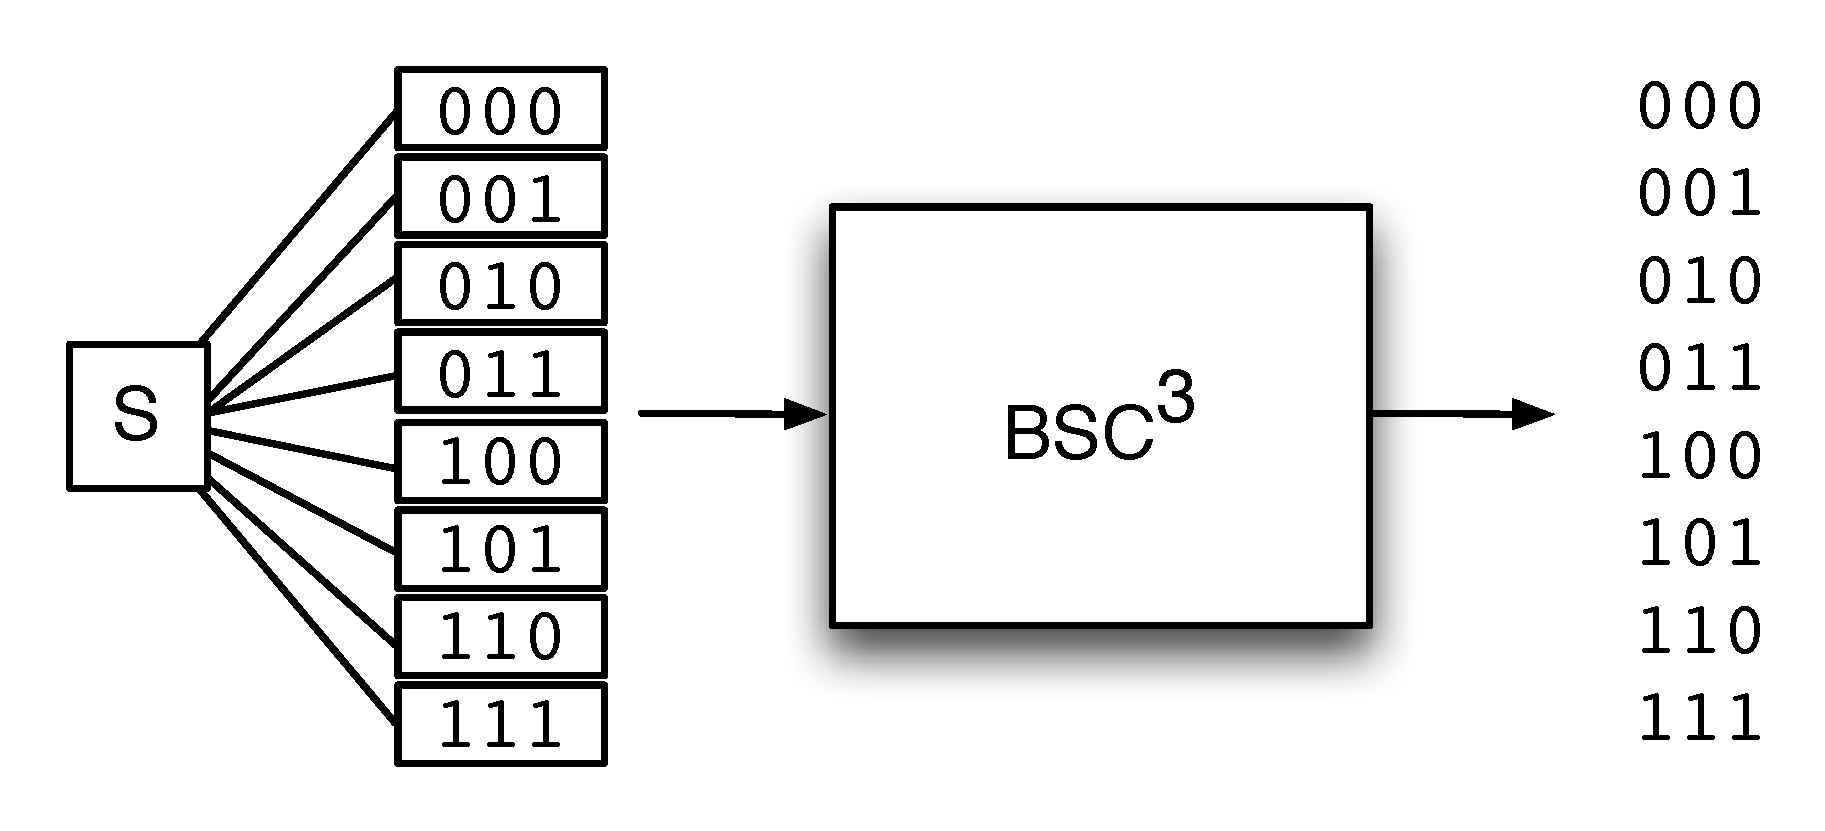
\includegraphics[width=0.6\textwidth]{img/mbsc1.pdf}
\caption{$BSC^3$ con M=8}
\label{fig:mbsc1}
\end{center}
\end{figure}

\begin{figure}[htbp]
\begin{center}
	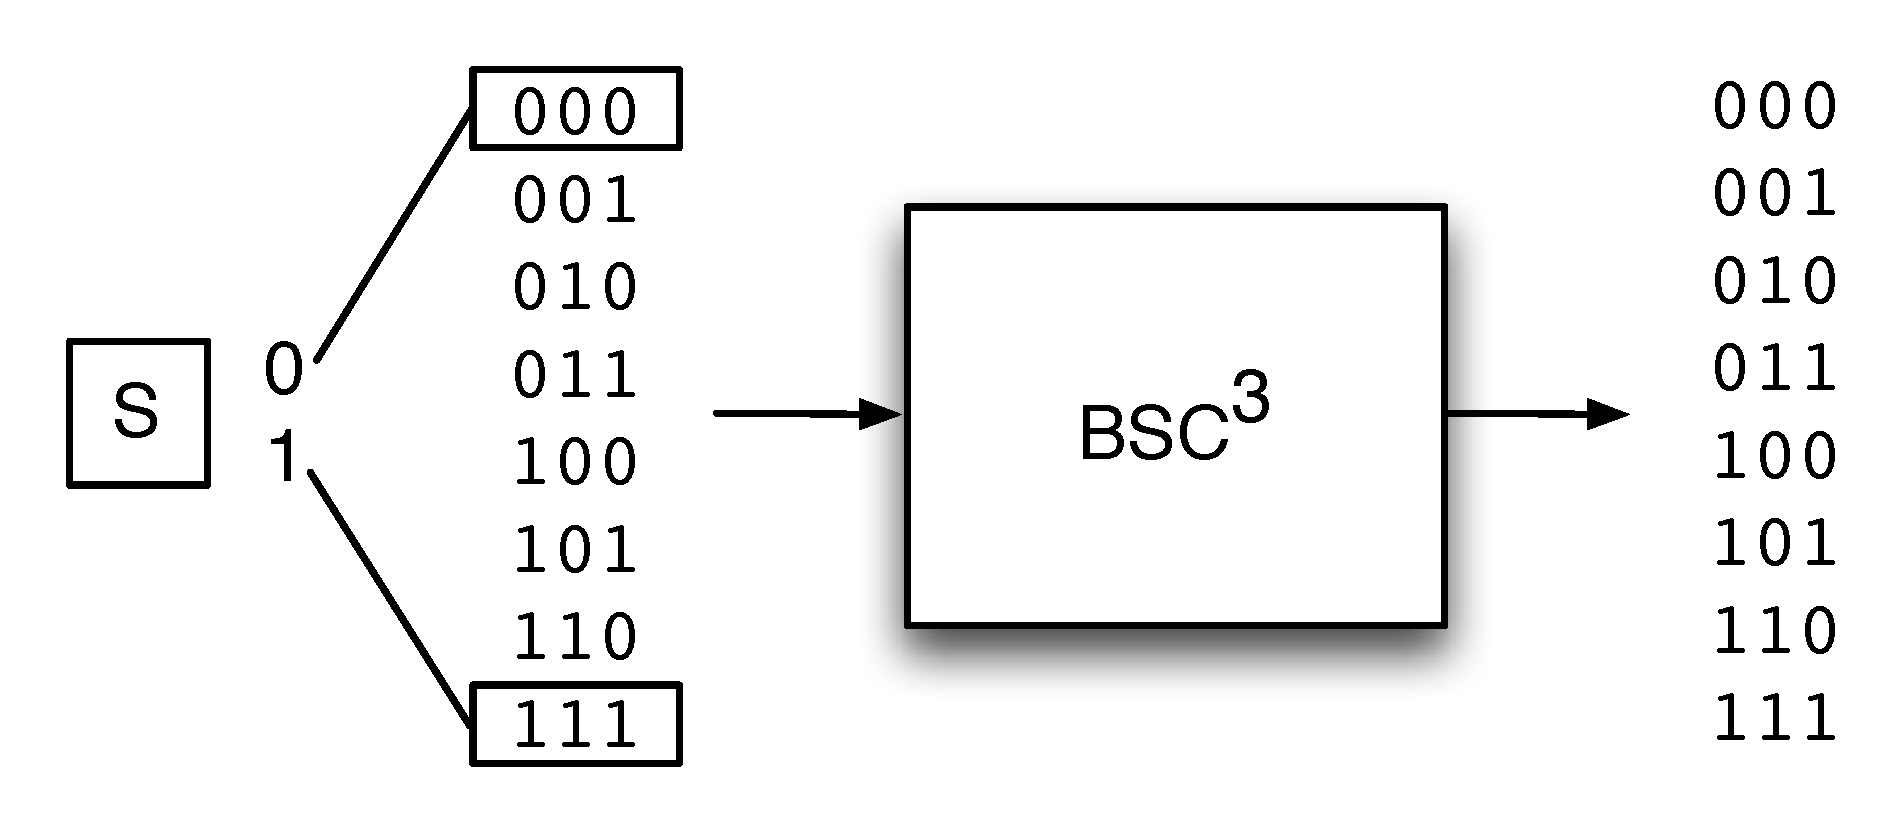
\includegraphics[width=0.6\textwidth]{img/mbsc2.pdf}
\caption{$BSC^3$ con M=2}
\label{fig:mbsc2}
\end{center}
\end{figure}

\begin{figure}[htbp]
\begin{center}
	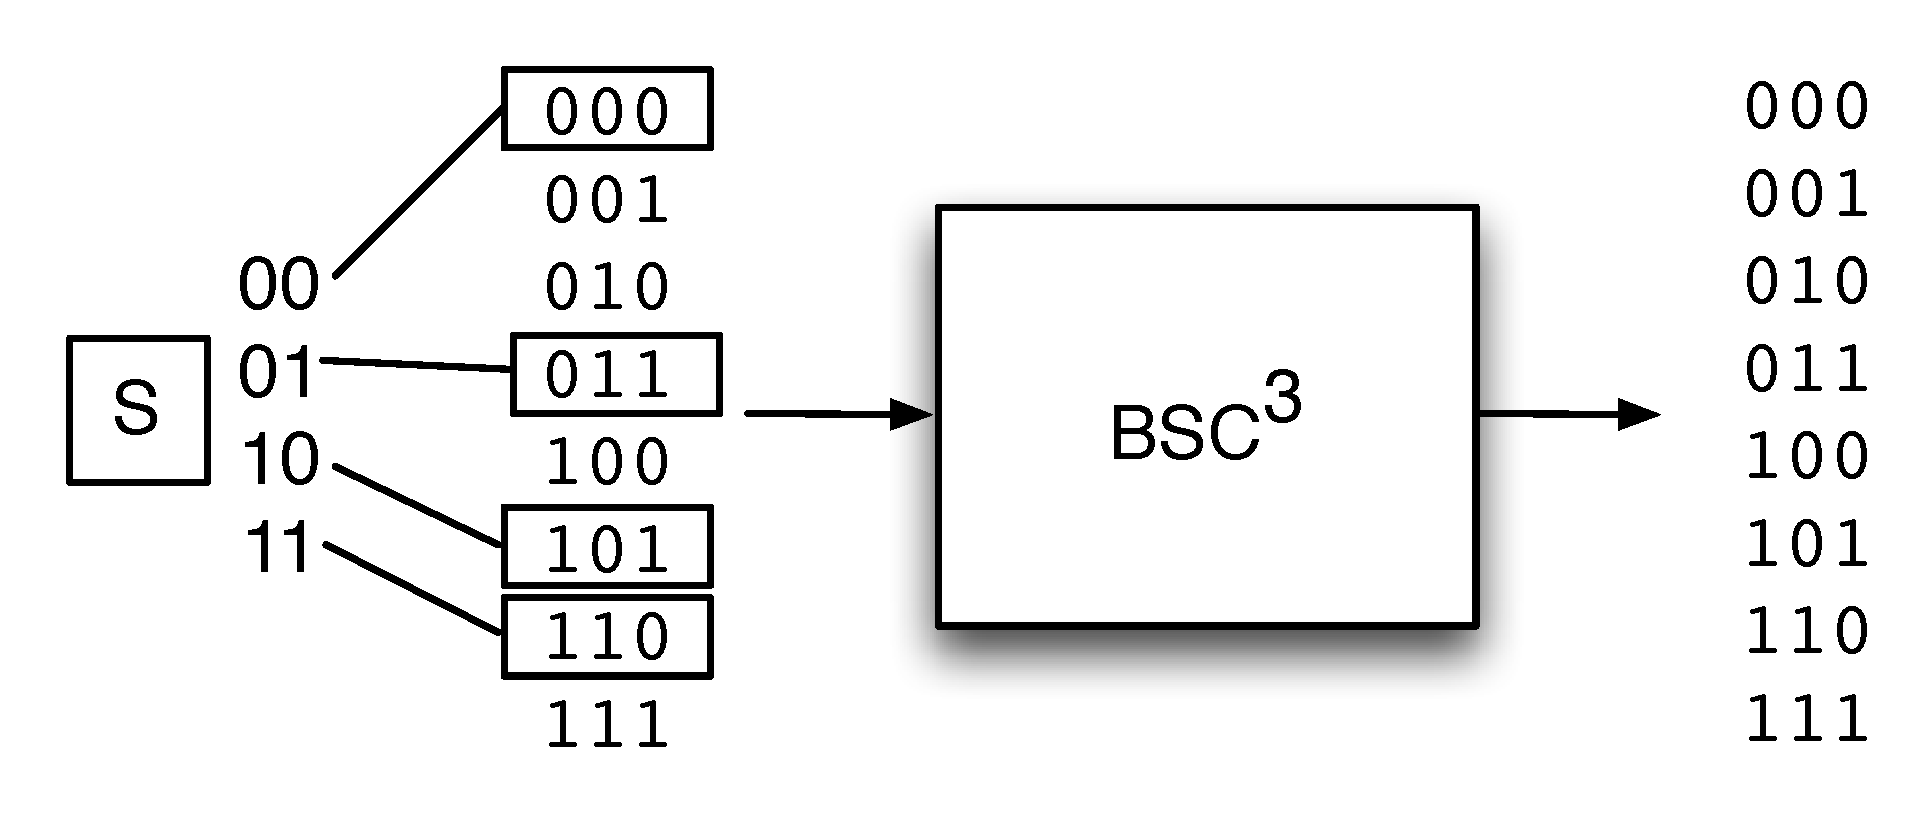
\includegraphics[width=0.6\textwidth]{img/mbsc3.pdf}
\caption{$BSC^3$ con M=4}
\label{fig:mbsc3}
\end{center}
\end{figure}

\newpage
\noindent
La funzione di decodifica per quest'ultimo caso è la seguente:
\[\begin{split}
 &d(000)=d(001)=00  \\
 &d(010)=d(011)=01  \\
 &d(100)=d(101)=10  \\
 &d(110)=d(111)=11  \\
 \end{split}
\]
Per scegliere i simboli da inviare sul canale, si può utilizzare il concetto di distanza di Hamming:
\begin{definizione}[Distanza di Hamming]
La distanza di Hamming tra due parole di codice (di uguale lunghezza) è il numero di posizioni in cui i 
simboli delle due parole differiscono.
\end{definizione}

Per esempio 000 e 011 hanno distanza di Hamming pari a 2 (gli ultimi 2 bit differiscono). Le parole di codice da inviare sono 
quindi state scelte al fine di massimizzare la distanza di Hamming tra le varie parole. Si nota infatti che la minima distanza in 
questo caso tra due parole qualsiasi è 2. In questo modo è possibile ``distanziare'' il più possibile le parole di codice, in maniera che errori sui singoli bit non transformino una parola di codice in un'altra.

Variando i due parametri che abbiamo considerato finora: l'estensione n del canale e le parole di codice inviabili M possiamo ottenere moltissimi codici (detti codici (M,n)).

\begin{definizione}[Codice di canale $(M,n)$]
Un codice di canale $(M,n)$ con:
\begin{itemize}
 \item n Estensione del canale
 \item M Numero di parole di codice inviabili sul canale
\end{itemize}
Si compone di:
\begin{itemize}
 \item Un index set $\{1,2,...,M\}$
 \item Una funzione di codifica $X^n: \{1,2,...,M\} \to X^n$
 \item Una regola di decisione d: $y^n \to \{1,2,...,M\}$
\end{itemize}

\end{definizione}

\begin{osservazione}
 Dato un codice $(M,n)$ il suo transmission rate è:
\[
 R=\frac{log(M)}{n}
\]

\end{osservazione}

\section{2° Teorema di Shannon}
Supponiamo di voler inviare un insieme n tendente ad infinito, di parole di codice in un canale. Nel codice a ripetizione che abbiamo visto nel paragrafo precedente, eravamo in grado di ridurre arbitrariamente la probabilità di errore. Tuttavia avevamo visto che ciò 
portava ad una riduzione del transmission rate. Nel caso limite in cui la probabilità di errore tendeva a 0, anche la velocità di trasmissione tendeva a 0.
L'importante risultato del secondo teorema di Shannon dimostra invece che è possibile ridurre arbitrariamente la probabilità di errore, 
purché il transimission rate sia inferiore alla capacità di canale. In altre parole scelto un transmission rate a piacere (più piccolo della capacità di canale) si potrà trasmettere con una probabilità di errore tendente a 0.

Per vedere in maniera intuitiva che ciò è vero, consideriamo i risultati visti nel paragrafo relativo all'AEP (vedi par. \ref{aep}).
Supponiamo di poter inviare sul canale le parole di codice $X_1..X_M$. Per ciascuna di esse, il destinatario può ricevere qualsiasi 
sequenza di $Y^n$, tuttavia per il teorema AEP nella quasi totalità dei casi saranno ricevute solamente delle sequenze tipiche.
Possiamo quindi pensare intuitivamente per ogni parola di codice inviata, le sequenze ricevute siano solamente quelle comprese in una 
``sfera''. Il numero di sequenze in ogni sfera (sempre per l'AEP) è circa $2^{n H(Y/X)}$. Avremo quindi $M$ sfere (una per ogni parola di codice), ciascuna con $2^{n H(Y/X)}$ sequenze. La situazione è quindi quella rappresentata in figura \ref{fig:sha2}.

\begin{figure}[htbp]
\begin{center}
	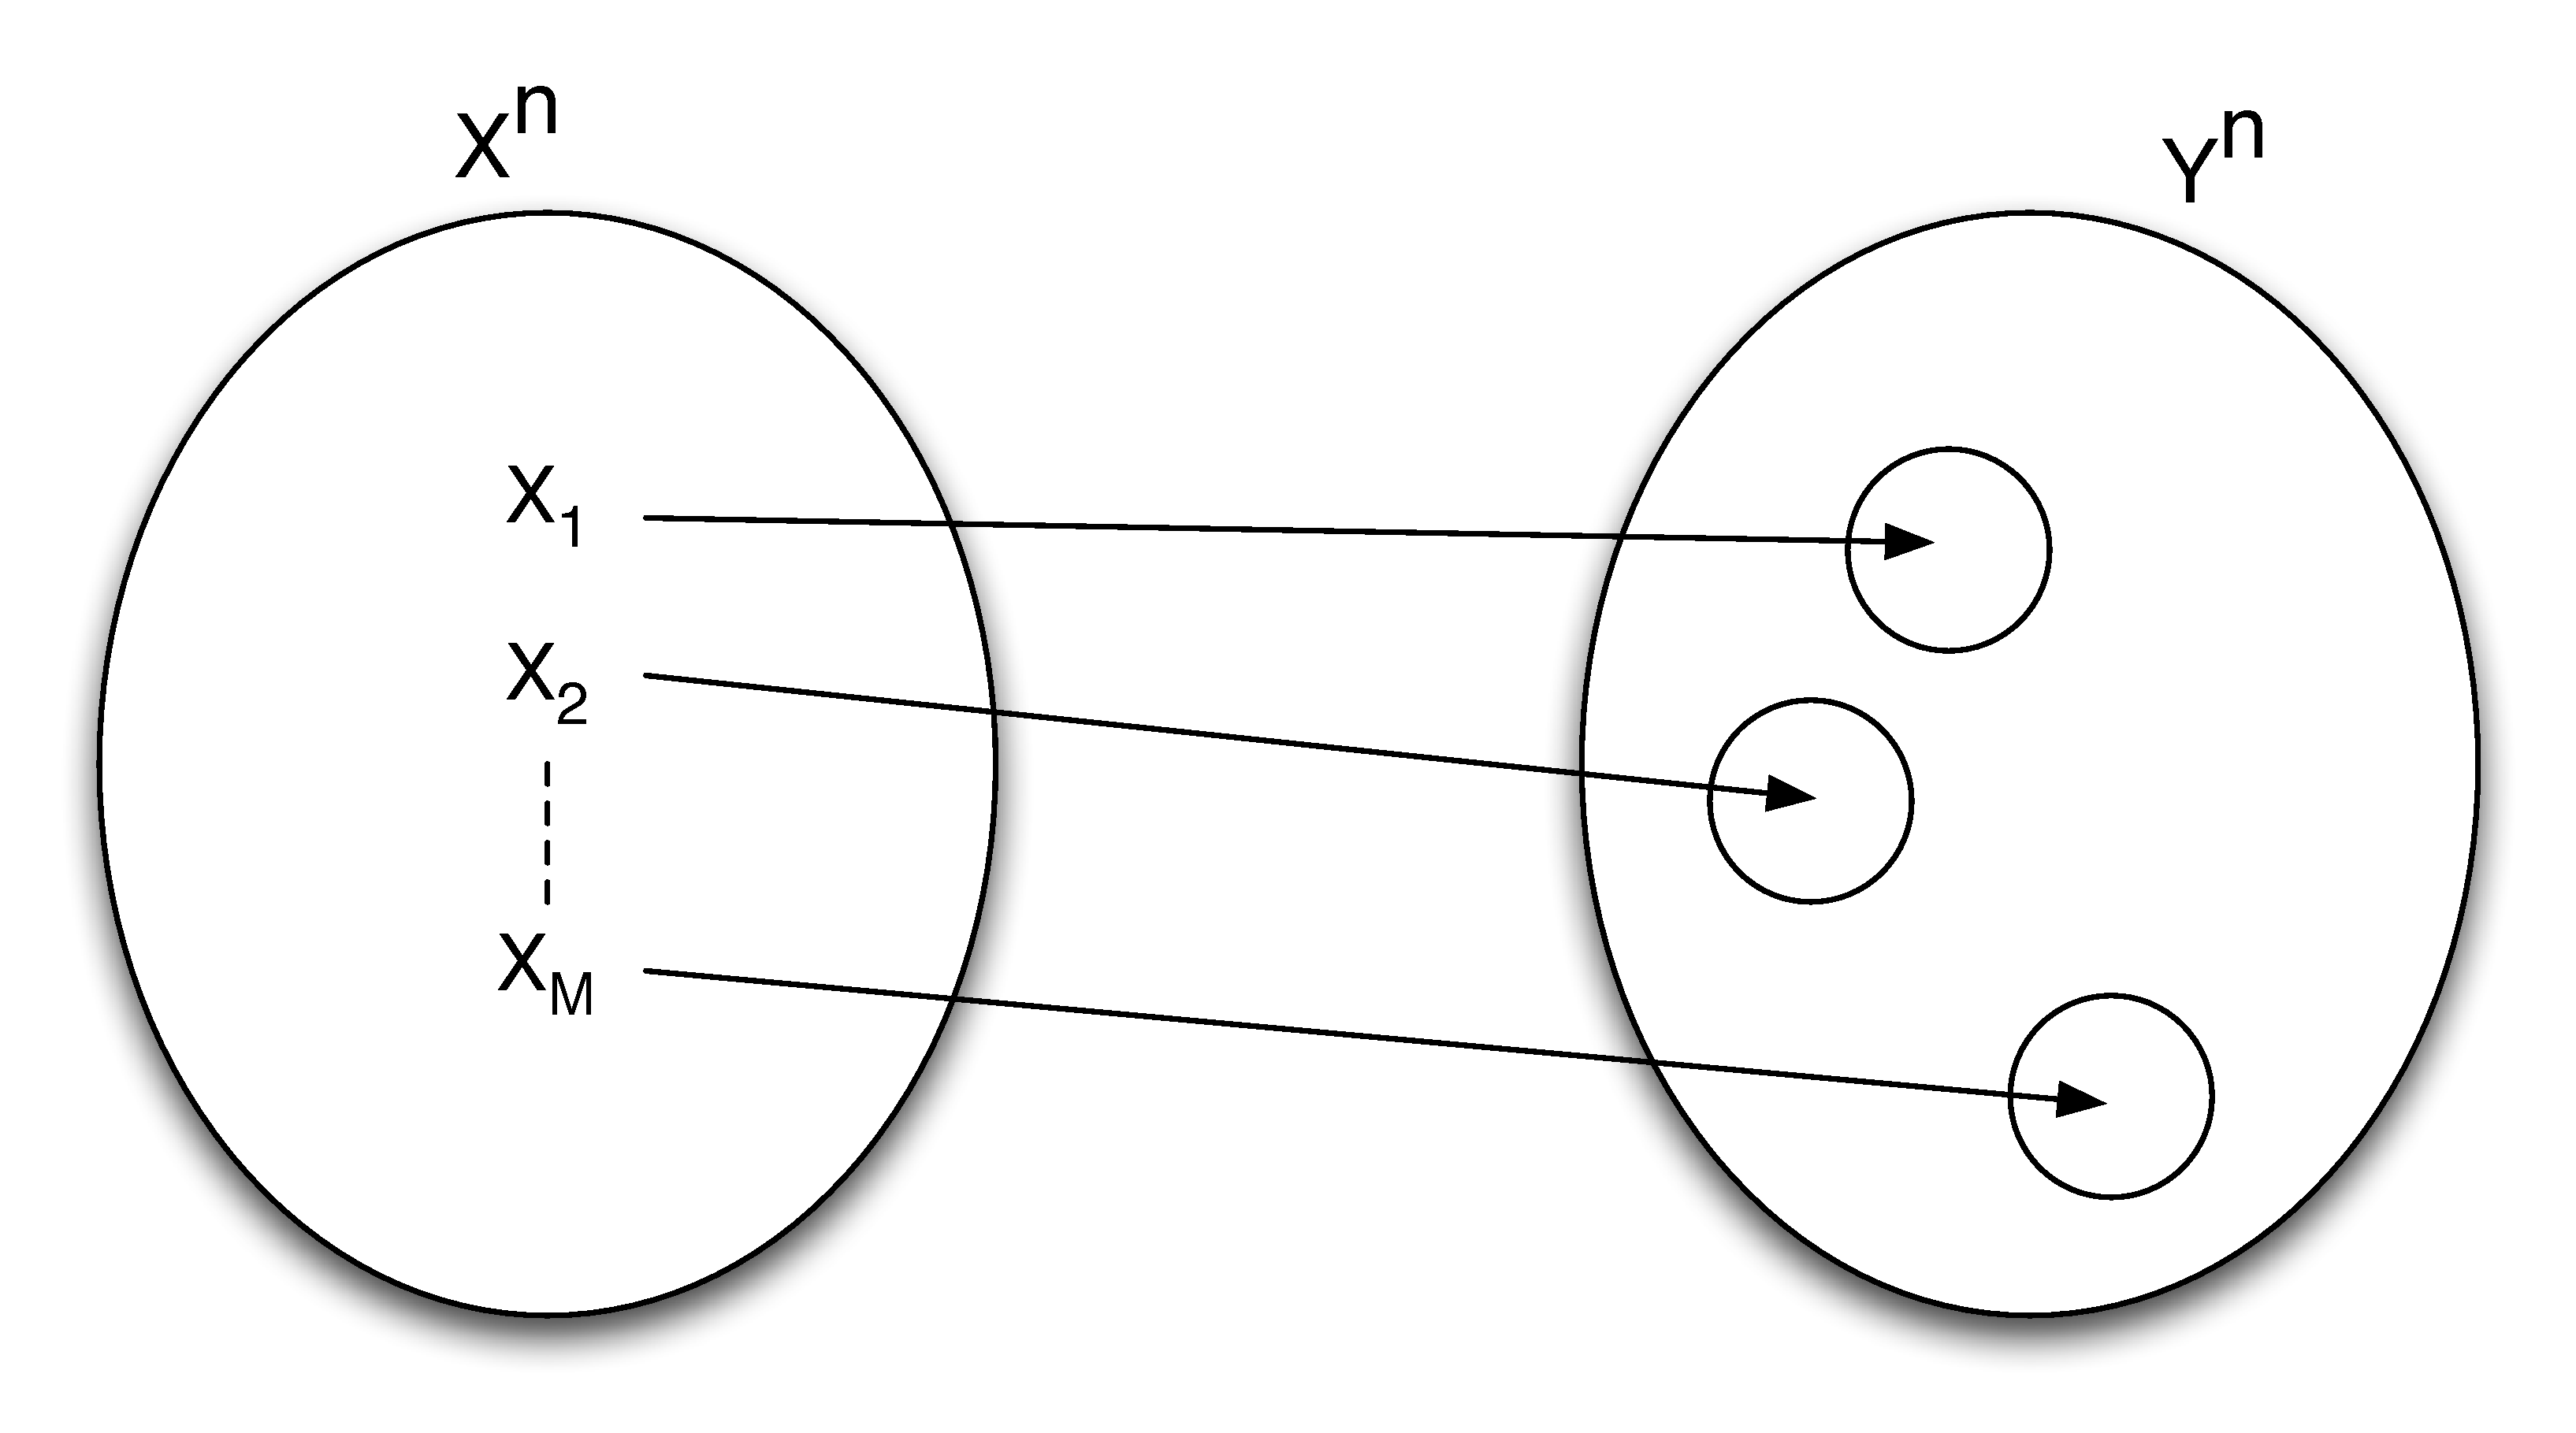
\includegraphics[width=0.6\textwidth]{img/sha2.pdf}
\caption{Rappresentazione intuitiva delle parole di codice inviate e delle sfere con le sequenze ricevute}
\label{fig:sha2}
\end{center}
\end{figure}

Si ponga ora attenzione al fatto che il numero totale di sequenze non è $M \times 2^{n H(Y/X)}$. Infatti non è detto che
le sfere siano tutte disgiunte. Il numero totale di sequenze tipiche è invece circa $2^{n H(Y)}$ (sempre per l'AEP). 
Ma sapendo quante sequenze contiene ogni sfera, possiamo ricavare il numero massimo di sfere possibili, affinché esse non si intersichino:
\[\begin{split}
 n_{max}&=\frac{2^{n H(Y)}}{2^{n H(Y/X)}} \\
    &=2^{n (H(Y)-H(Y/X))} \\
    &=2^{n I(X;Y) }
  \end{split}
\]

Ma per avere una trasmissione affidabile, siamo proprio interessati al fatto che non ci sia intersezione tra le sfere. In caso contrario infatti per una sequenza che fa parte di due sfere, si avrebbero più parole di codice possibili tra cui scegliere. Il numero M di sfere, deve essere quini inferiore ad $n_{max}$, per essere in grado di determinare la parola 
di codice inviata.
Deve quindi essere:
\[\begin{split}
 M \le & 2^{n I(X;Y)} \\
  log(M) \le & n I(X;Y) \\
 \frac{log(M)}{n} \le & I(X;Y) \\
 R \le & I(X;Y) \\
 R \le & I(X;Y) \le C \\
 R \le & C \\
  \end{split}
\]

\bigskip

Passiamo ora alla formulazione e dimostrazione vera e propria del teorema. Al solito, presentiamo prima alcuni risultati utili per la dimostrazione. Innanzitutto introduciamo il concetto di canali in cascata. Dati due canali $C_1$ e $C_2$, possiamo infatti porli appunto ``in cascata'', ovvero uno di seguito all'altro. La situazione è quella rappresentata in figura \ref{fig:cascata}. E' possibile indicare (riferendoci ai simboli usati in figura) che i canali sono in cascata con $X \to Y \to Z$.

\begin{figure}[htbp]
\begin{center}
	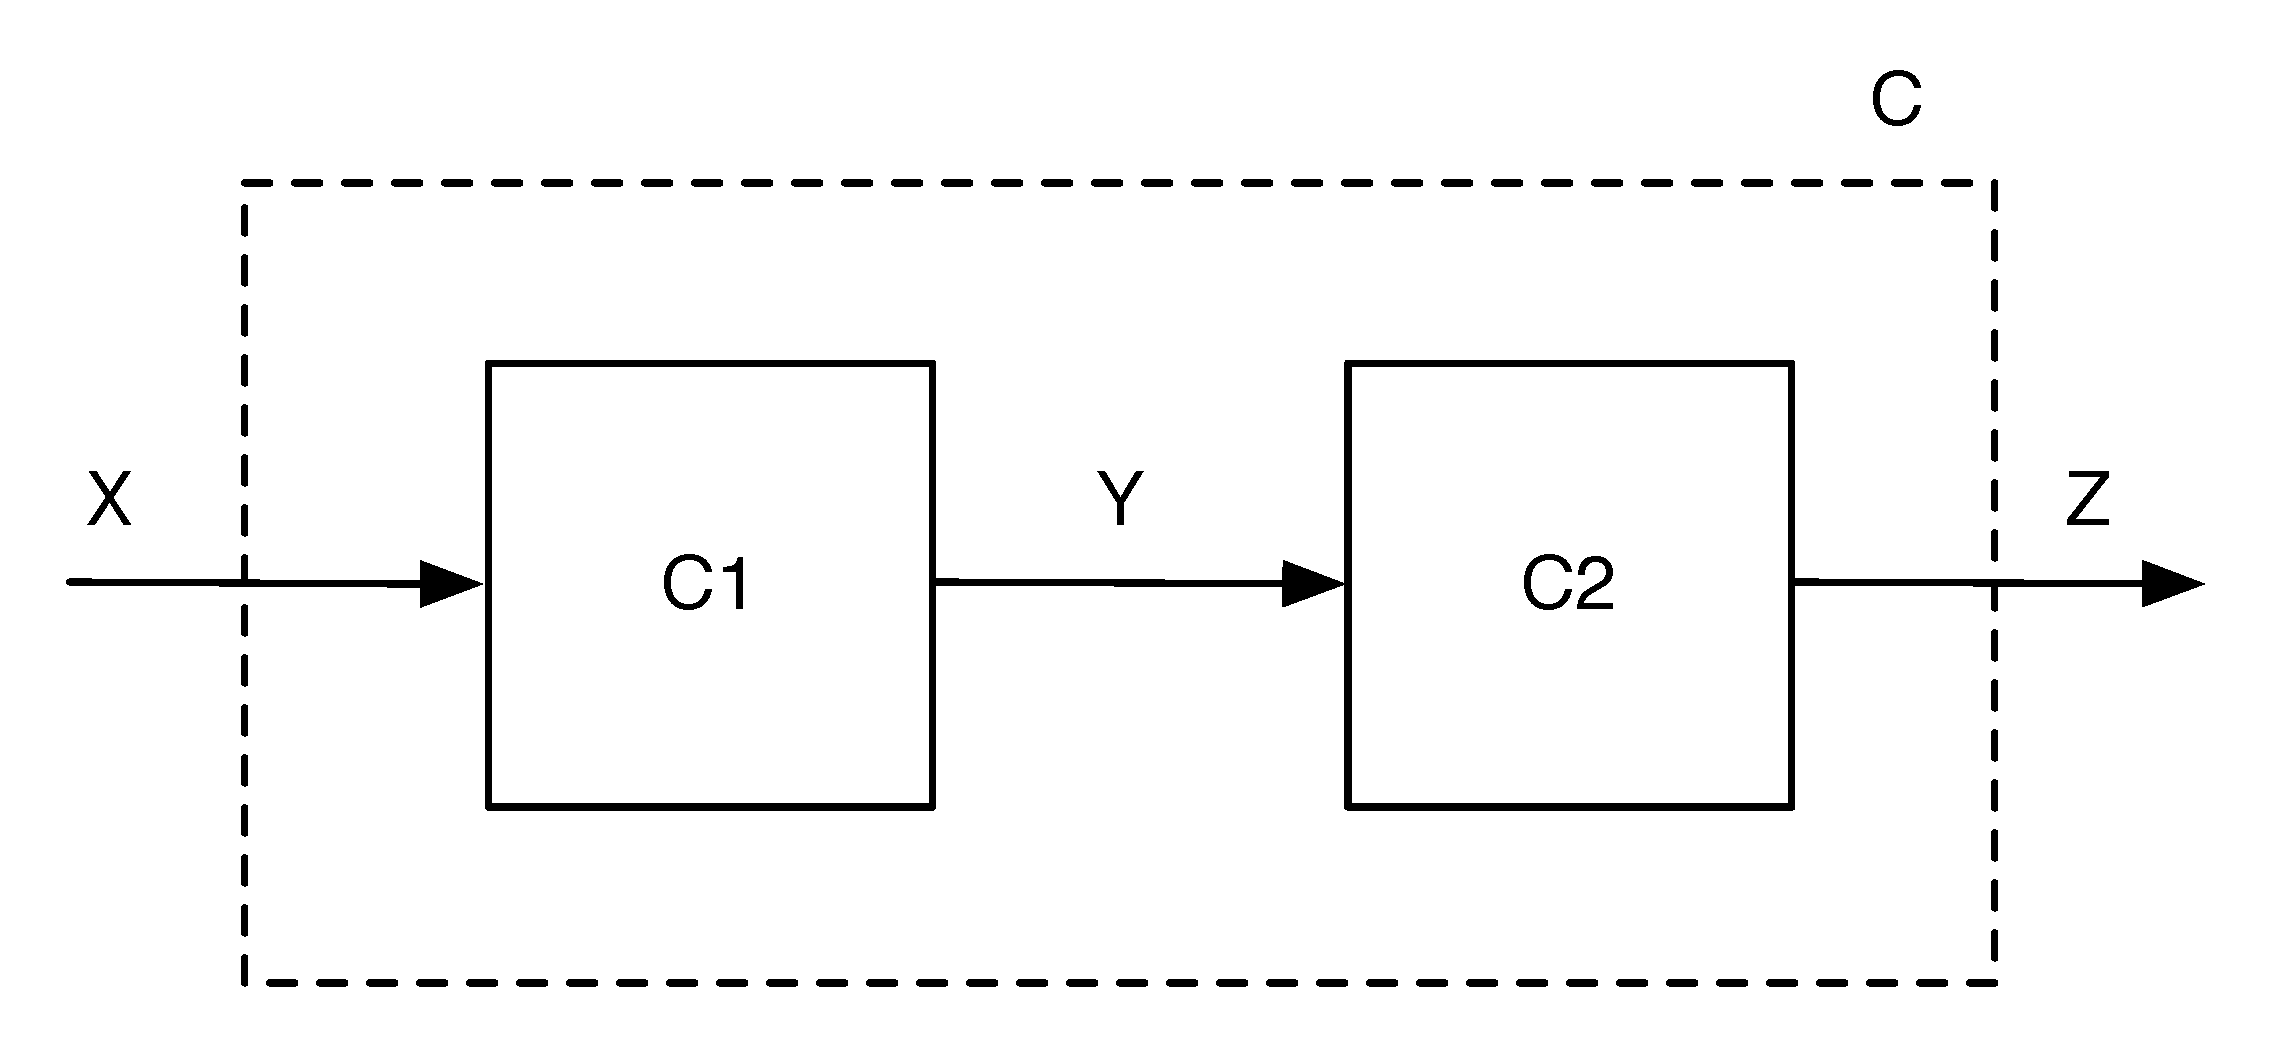
\includegraphics[width=0.6\textwidth]{img/cascata.pdf}
\caption{Due canali in cascata}
\label{fig:cascata}
\end{center}
\end{figure}

E' interessante determinare la matrice di canale che si ottiene ponendo in cascata due canali $C_1$ e $C_2$. In maniera abbastanza semplice, si nota come tale matrice è il prodotto delle matrici di canale di $C_1$ e $C_2$, ovvero $P=P_1 \times P_2$. Per fare un esempio consideriamo due canali BSC, rispettivamente con matrici di canale P1 e P2:

\[ P_1 = \left[
  \begin{array}{cc}
    1-p_1 & p_1 \\
    p_1 & 1-p_1 \\
  \end{array} \right]
  \\
  P_2 = \left[
  \begin{array}{cc}
    1-p_2 & p_2 \\
    p_2 & 1-p_2 \\
  \end{array} \right]
\]

Allora la matrice $P$, del canale che si ottiene ponendoli in cascata è:
\[
 P = \left[
  \begin{array}{cc}
    (1-p_1)(1-p_2) + p_1 p_2 & (1-p_1)p_2 + p_1(1-p_2) \\
    p_1 (1-p_2)+(1-p_1)p_2 & p_1 p_2 +(1-p_1)(1-p_2)\\
  \end{array} \right]
\]

\begin{figure}[htbp]
\begin{center}
	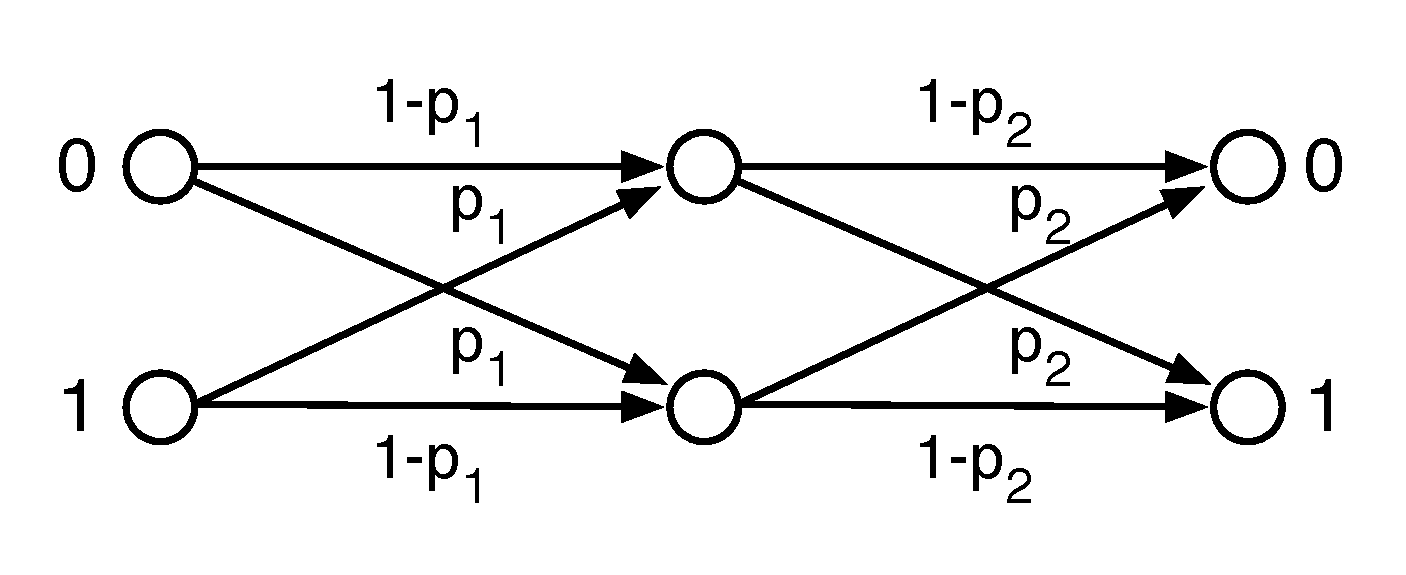
\includegraphics[width=0.6\textwidth]{img/cascata2.pdf}
\caption{Due BSC in cascata}
\label{fig:cascata2}
\end{center}
\end{figure}

\bigskip



\begin{lemma}
\mbox{}

Dati due canali in cascata $X \to Y \to Z$:
 \begin{itemize}
  \item $p(z/y,x)=p(z/y)$
  \item $p(x/y,z)=p(x/y)$
 \end{itemize}
 \begin{proof}
  Dimostriamo solo la seconda uguaglianza:
  \[\begin{split}
   p(x/y,z)=& \frac{p(y,z/x)p(x)}{p(y,z)} \\
   =&\frac{p(z/x,y)p(y/x)p(x)}{p(z/y)p(y)} \\
   =&\frac{p(z/y)p(y/x)p(x)}{p(z/y)p(y)} \\
   =&\frac{p(y/x)p(x)}{p(y)} \\
   =&p(x/y)
    \end{split}
  \]

 \end{proof}
\label{lem:cascata}
\end{lemma}

\begin{teorema}[Disuguaglianza dell'elaborazione dati]
\mbox{}

Dati due canali in cascata $X \to Y \to Z$:
 \begin{itemize}
  \item $I(X;Y) \ge I(X;Z)$
  \item $I(Y;Z) \ge I(X;Z)$
 \end{itemize}
\begin{proof}
 Dimostriamo solo la prima disuguaglianza.
 \[
  I(X;Y)=H(X)-H(X/Y)
 \]
 E:
 \[
  I(X;Z)=H(X)-H(X/Z)
 \]
 Quindi dimostrare che $I(X;Y) \ge I(X;Z)$, equivale a dimostrare che:
 \[\begin{split}
  & H(X)-H(X/Y) \ge H(X)-H(X/Z) \\
  \iff & -H(X/Y) \ge -H(X/Z) \\
  \iff & H(X/Y) \le H(X/Z) \\
  \iff & H(X/Y)-H(X/Z) \le 0 \\
  \iff & H(X/Z)-H(X/Y) \ge 0 \\
   \end{split}
 \]
Ora:
\[\begin{split}
  & H(X/Z)-H(X/Y)= \\
 =&\sum_{x \in X} \sum_{z \in Z} p(x,z) log \frac{1}{p(x/z)} - \sum_{x \in X} \sum_{y \in Y} p(x,y) log \frac{1}{p(x/y)} \\
 =&\sum_{x \in X} \sum_{z \in Z} log \frac{1}{p(x/z)}  \sum_{y \in Y} p(x,y,z) 
  - \sum_{x \in X} \sum_{y \in Y} log \frac{1}{p(x/y)} \sum_{z \in Z} p(x,y,z) \\
 =&\sum_{x \in X} \sum_{y \in Y} \sum_{z \in Z} p(x,y,z) log \frac{1}{p(x/z)} 
  - \sum_{x \in X} \sum_{y \in Y} \sum_{z \in Z} p(x,y,z) log \frac{1}{p(x/y)} \\
 =&\sum_{x \in X} \sum_{y \in Y} \sum_{z \in Z} p(x,y,z) log \frac{p(x/y)}{p(x/z)} \\
  \end{split}
\]
Ma per il lemma \ref{lem:cascata} $p(x/y)=p(x/y,z)$, quindi:
\[\begin{split}
  &\sum_{x \in X} \sum_{y \in Y} \sum_{z \in Z} p(x,y,z) log \frac{p(x/y)}{p(x/z)} \\
 =&\sum_{x \in X} \sum_{y \in Y} \sum_{z \in Z} p(x,y,z) log \frac{p(x/y,z)}{p(x/z)} \\
 =&\sum_{x \in X} \sum_{y \in Y} \sum_{z \in Z} p(y,z) p(x/y,z) log \frac{p(x/y,z)}{p(x/z)} \\
 =&\sum_{y \in Y} \sum_{z \in Z} p(y,z) \sum_{x \in X} p(x/y,z) log \frac{p(x/y,z)}{p(x/z)} \\
 \ge & 0
 \end{split}
\]
L'ultimo passaggio deriva dal fatto che $p(y,z)$ è una probabilità (e quindi maggiore uguale a 0), mentre il 
secondo termine è una distanza di Kullback-Leibler, che per il teorema \ref{leibler} è maggiore o uguale a 0.
\end{proof}
\end{teorema}

\medskip

La disuguaglianza dell'elaborazione dati dice in sostanza che l'informazione mutua, man mano che si attraversano dei canali, 
non può aumentare. In sostanza ad ogni ``passaggio'' si può solo perdere informazione (e mai guadagnarne).

\bigskip

\begin{teorema}[Disuguaglianza di Fano]
\mbox{}

Siano $X,Y$ variabili casuali e $g(Y)=\widehat{X}$ una regola di decisione. Sia:
\[
 P_E=P\{\widehat{X} \neq X\}
\]
Allora:
\[
 H(X/Y) \le H(P_E)+P_E log(|X|-1)
\]
\begin{proof}
\mbox{}

 Costruiamo una nuova variabile casuale E, nel seguente modo:
 \[
  E=
  \begin{cases}
    1 & \widehat{X} \neq X \\
    0 & \widehat{X}=X \\
  \end{cases}
 \]
 Allora:
 \[\begin{split}
   H(X/Y)=&H(X/Y)+H(E/X,Y) \\
         =&H(E,X/Y) \\
         =&H(E/Y)+H(X/E,Y) \\
         \le & H(E) + H(X/E,Y) \\
         = & H(P_E) + H(X/E,Y) \\
   \end{split}
 \]

Il primo passaggio deriva dal fatto che $H(E/X,Y)=0$ in quanto se si conoscono $X$ e $Y$, allora banalmente si conosce anche $E$. 
Il secondo e il terzo sono applicazioni 
della regola della catena (in particolare corollario del teorema \ref{catena}). Il quarto passaggio 
deriva dal fatto che il condizionamento riduce l'entropia (osservazione \ref{condizionamento}).
Ora:
\[\begin{split}
 H(X/E,Y) =&Pr\{E=0\}H(X/Y,E=0)+
           Pr\{E=1\}H(X/Y,E=1) \\
          =&Pr\{E=0\} \cdot 0 + Pr\{E=1\}H(X/Y,E=1) \\
          =&Pr\{E=1\}H(X/Y,E=1) \\
          =&P_E H(X/Y,E=1) \\
          \le& P_E log(|X|-1)
  \end{split}
\]
L'ultimo passaggio deriva dal fatto che il massimo valore che può raggiungere l'entropia è il logaritmo del 
numero di simboli. Ma se E=1 allora $\widehat{X}\neq X$, quindi ho qualche informazione in più sul simbolo inviato. 
Ovvero so che non sarà $\widehat{X}$. Rimane dunque da ``scegliere'' tra $|X|-1$ simboli, la cui massima entropia è proprio 
$log(|X|-1)$.
Riassumendo:
\[
 H(X/Y) \le H(P_E) + H(X/E,Y) \le H(P_E)+P_E log(|X|-1)
\]
Che conclude la dimostrazione
\end{proof}
\end{teorema}

\begin{corollario}
 \[
  H(X/Y) \le 1+P_E log(|X|)
 \]
\begin{proof}
 Segue direttamente dal teorema:
 \[\begin{split}
 H(X/Y) & \le H(P_E)+P_E log(|X|-1) \\
        & \le log(2) + P_E log(|X|-1) \\
        & \le 1 + P_E log(|X|)
  \end{split}
 \]
\end{proof}
\end{corollario}


\begin{lemma}
 Sia $C=(X,p(y/x),Y)$ un canale senza memoria e sia 
$C^n=(X^n,p^n(x,y),Y^n)$ la sua estensione n-esima. Allora:
\[
 I(X^n;Y^n) \le nC
\]
\begin{proof}
 \mbox{}
Ricordando che se C è senza memoria:
\[
p(y^n/x^n)=\prod_{i=1}^n p(y_i,x_i) 
\]
Si ha:
\[\begin{split}
 I(X^n;Y^n) &=H(Y^n)-H(Y^n/X^n) \\
 & = \sum_{i=1}^n H(Y_i/Y_1,Y_2,...,Y_{i-1}) - H(Y^n/X^n) \\
 & \le \sum_{i=1}^n H(Y_i) - H(Y^n/X^n) \\
 & \le \sum_{i=1}^n H(Y_i) - \sum_{i=1}^n H(Y_i/Y_1,Y_2,...,Y_{i-1},X^n) \\
 & = \sum_{i=1}^n H(Y_i) - \sum_{i=1}^n H(Y_i/X_i) \\
 & = \sum_{i=1}^n  [ \ H(Y_i)- H(Y_i/X_i) \  ] \\
 & = \sum_{i=1}^n I(X_i;Y_i) \\
 & \le nC
  \end{split}
\]
\end{proof}
Il secondo e il quarto passaggio seguono dalla regola della catena (generalizzata).
Il terzo passaggio segue invece dal fatto che il condizionamento riduce l'entropia (oss. \ref{condizionamento}).
Il quinto passaggio deriva dal fatto che il canale è senza memoria.
L'ultimo passaggio, infine, deriva dal fatto che la capacità di canale è il massimo dell'informazione mutua.
\label{lsh}
\end{lemma}


\bigskip

\noindent
Possiamo ora enunciare e dimostrare una parte del 2° teorema di Shannon.

\begin{teorema}[2° teorema di Shannon (o della codifica di canale)]
 \mbox{}

 \begin{enumerate}
  \item Sia $A=(X,p(y/x),Y)$ un canale con capacità $C$ e sia $R \le C$.

        \noindent
        Allora esiste una sequenza di codici $(2^{nR},n)$ tali che:
        \[
         P_E^{(n)} \xrightarrow[n \to \infty]{} 0
        \]
        Ovvero:
        \[
         \forall \epsilon>0, \exists n_0 \in N: \forall n \ge n_0 \ P_E^{(n)}< \epsilon
        \]
   \item Se esiste una sequenza di codici $(2^{nR},n)$, tali che:
         \[
          P_E^{(n)} \xrightarrow[n \to \infty]{} 0
         \]
         Allora $R \le C$
 \end{enumerate}
 \begin{proof}
  \mbox{}
  \begin{description}
   \item[1.] Omesso, la dimostrazione è complicata.
   \item[2.] 
    
    Indichiamo con $W$ l'insieme delle parole di codice inviabili sul canale.
    Quindi:
    \[
     W \to X^n(W) \to Y^n
    \]
    \noindent
    Poiché stiamo considerando dei codici $(2^{nR},n)$, si avrà:
    \[
     |W|=2^{nR}
    \]
    Quindi, poiché consideriamo le parole di codice tutte equiprobabili, si avrà:
    \[
     H(W)=log(|W|)=log(2^{nR})=nR
    \]
   Da cui:
   \[\begin{split}
    nR=H(W)&=H(W/Y^n)+I(W;Y^n) \\
        & \le H(W/Y^n)+I(X^n;Y^n) \\
        & \le H(W/Y^n)+nC \\
        & \le 1+P_E^{(n)} log(|W|) +nC \\
        & = 1+P_E^{(n)} nR +nC \\
     \end{split}
   \]
   Il secondo passaggio deriva dalla disuguaglianza dell'elaborazione dati, il terzo invece dal lemma \ref{lsh}.
   Il quarto passaggio segue dal corollario alla disuguaglianza di Fano.

   Ora dividendo ambo i membri per n si ottiene:
   \[
    R \le \frac{1}{n}+P_E^{(n)} R +C
   \]
   Ma:
   \[
    \lim_{n \to \infty} \frac{1}{n}+P_E^{(n)} R +C=C
   \]
   Da cui:
   \[
    R \le C
   \]

  \end{description}

 \end{proof}

\end{teorema}
